

\chapter{Three models of the medium}\label{ch:medium}



\section{Introduction}
Physically correct models of a fluid medium predict a non-constant signal speed for two reasons,
\begin{enumerate}
\item the self-advection of the medium,
\item local perturbations in density and temperature that in turn affect the speed of sound locally.
\end{enumerate}
These predictions are at odds with what can be measured with ultrasound.
To model the outcome of an ultrasound experiment one must recognise from the outset the distinction between what is measured and what is physically correct.

Both sources of variance in the signal speed become vanishingly small if the disturbance is small.
In this case the disturbance propagates at a fixed speed according to the linear wave equation.
A fluid that is only perturbed slightly is therefore conformant with the requirements of acoustic measurement.
One expects, therefore,
that the acoustic model and the correct model converge in this limit.
If a disturbance is localised, then in the far field acoustic measurement makes correct measurements.

We therefore have a starting point for our acoustic model.
If we were assert that ultrasound - due to the incorrect assumption of a constant sound speed - measures linear fluids
then we have a model for acoustic measurement that is self-consistent.
This is a step forward over what is offered by the correct model.
%because in contrast with the correct model of the medium
%it enables distances within the fluid medium to be defined in a consistent manner with what is acoustically measured.
The predictive power of the linear model is explored in this first attempt of an acoustic model in \secref{linearFluid}.

Nonetheless, defining acoustic model as the small perturbation limit of the correct model is unsatisfactory.
There is nothing within the theory that states the perturbations should be small,
and so insisting that non-negligible perturbations should be neglected in order to keep the
theory self-consistent is wrong.
An improvement is given in the second attempt of an acoustic model in \secref{incompressibleFluid}.
In this model the dynamics of the fluid are chosen to match the physically correct theory through the Euler equations and the continuity
equation,
but the equation of state is chosen in such a way as to enforce the constancy of the speed of sound.
There is a more comfortable feel about this approach as we are not modifying the fundamental physics in any way,
but rather placing the limitations of acoustic measurement in the degree to which the fluid probed can be understood.

There are still problems.
While the sound speed is set to be constant,
the self-advection of the fluid remains.
A linear wave equation can be recovered, but only in a local frame of reference taken to be stationary with the fluid.
In other frames the self-advection term contributes to a signal that can propagate at faster than the sound speed.
%
%While the equation of state can be chosen such that the speed of sound is constant,
%the self-advection of the fluid contributes to the signal travelling at faster than the sound speed.
%%
%
%Morevoer, the privaledge of a frame of motion where the fluid is locally stationary
When spatial locations are measured with sound signals,
the measurements of such motions are impossible.
A model cannot simultaneously be Lorentz invariant, with the sound speed being the limiting velocity,
and yet still admit supersonic speeds.
A Lorentz invariant model cannot admit such privileged frames of reference.
%This is contry to acoustic definition of space, where
%the measurement of motions faster than the speed of sound is impossible.
%
%the signal travelling 
%he limitations of acoustic measurement are therefore placed degree to which the medium can be understood, rather than due to the underling physics.
%
%Neither of these models are Lorentz invarient

In \secref{Maxwell} this short-cumming is corrected by using an equation of state that ensures a constant speed of sound in an Lorentz invariant framework.
It is found, appropriately given the constraints from acoustic measurement,
that the signal propagates according to the linear wave equation with a constant speed of sound.
This is our final model of the medium.

%These models build upon eachother, so we begin w


%Equations of state that are confirmed by other experimental techniques do not correctly predict the outcomes of ultrasound experiments
%due to ultrasound's incorrect reliance on a constant sound speed.


%It is at this point that the required constancy of the speed of sound poses some interpretation problems to the acoustic observer.




%for it is well known that the sound speed in a fluid is not in general constant.
%The sound speed is a function of the medium's thermodynamic quantities such as  density, pressure, temperature and entropy,
%and these vary throughout the fluid, not least due to the propagation of the sound wave itself.
%Equations of state that are confirmed by other experimental techniques do not correctly predict the outcomes of ultrasound experiments
%due to ultrasound's incorrect reliance on a constant sound speed.





%This is a difficult square to circle.

%One option would be to use ultrasound for the spatio-temporal location of entities, and then ascribe the real, independently measured physical properties and physical laws to those entities.



%One option would be to use ultrasound for the spatio-temporal location of entities, and then ascribe the real, independently measured physical properties and physical laws to those entities.
%An example would be modelling an acoustic medium as an ideal gas; the locations of echos described by \eqnref{radar} and the thermodynamic properties of the medium described by the ideal gas law.
%While this approach seems reasonable it suffers from a lack of internal consistency. 
%An ideal gas heats when compressed, and this alters the speed of sound.  
%Such physics is unmeasurable with ultrasound, even if the underlying model is correct.
%On the one hand the measurement processes assumes that the sound speed is fixed, 
%while on the other the properties of the medium imply that is not.  
%The measurements made with ultrasound will not agree with the predictions of a physically correct model due to ultrasound's reliance on assuming a constant sound speed.


%Put another way, 
%such an approach implies that ultrasound measurement alone cannot measure the properties ascribed in the model.  

%An alternative is to focus on modelling what is measurable - thereby insisting on the internal consistency of the physics.
%Since ultrasound requires that the speed of sound be constant as part of its measurement process, 
%the approach insists that the  model of the medium be consistent with this requirement.
%The equations of state are therefore determined by what can be measured acoustically, 
%rather than driven by what has been shown to be successful in other domains of physics.

%Both approaches are difficult to accept, 
%because in both we have to accept a distinction between 
%Such an approach refute 
%We show in \secref{nonlinear} that this implies that we model fluids with an the adiabatic index of unity.



%Consider for example the acoustic measurement of a compression of the gas in \figref{compression}.
%When the valve compresses the gas the  ideal gas is compressed, it heats up and this increases the speed of sound. 
%However, this change in sound speed is not reflected in the measurement process, and so the physical theory predicted 
%The acoustic measurement processes continues with the original sound speed and so the measured compression is incorrect.  
%The time it takes for a compression phase of the sound wave to return differs from that of the rarefaction.  


%The difficulty with this is that 

% to try to ensure that the underlying thermodynamic properties of the medium are
%If these thermodynamic properties are assumed to take their real, independently measured values then the implied local speed of sound will in general be different than the sound speed assumed in ultrasound.  
%Accordingly, the location where these perturbations are calculated - from their real values - differs from the location that is measured in ultrasound.  
%One would then have to maintain a mapping between what is measured acoustically, with a detailed knowledge of the medium so the real thermodynamic properties can be maintained correct.
%If such a detailed knowledge of the measured medium exists, then the need for acoustic measurement at all is deminished.




%The measured locations of these perturbations will then differ from where the fluctuation actually occured.  In short, we have a contradiction - we ascribe a   valuesare measured independently from the acoustic properties of the medium, 
%then these properties will imply 



\section{First attempt: A linear medium}\label{sec:linearFluid}

%A natural point to start is to assume that the physical description of the medium does not depend on the imaging modality.
%As an example, let us suppose that we are conducting an ultrasound experiment where we are propagating sound through an ideal gas.
%The pressure, $p$, density, $\rho$ and temperature, $T$, are therefore modelled by the ideal gas equation
%\eq{
%  p = \rho R T,
%}
%where $R$ is the specific gas constant.

A linear medium, where only first order perturbations to density and fluid velocity are considered,
has the properties required for a model of acoustic measurement.
The sound speed is constant and self-advection is ignored to this degree of approximation,
and so medium supports a signal that propagates with a constant sound speed.
Furthermore, a linearised medium approximates well the correct model of the medium far from a perturbation.

While it is not justifiable to suggest that ultrasound measures a linearised medium,
it is still worthwhile to understand how the linear wave equation is recovered,
and how the sound speed relates to the thermodynamics of the medium.

We begin, therefore, with the continuity equation and Euler equation that define the conservation of mass and momentum, respectively,
in the fluid:
%
%
%As a first question, let us then ask how these properties change in the medium in response to the sound wave.
%To understand the dynamics of the system we use our starting assumption a second time and model the dynamics of the gas with the Euler equation and continuity equation.
%Ignoring viscous effects, we then have\todo{Use hat notation for actual quantities},
\sub{
\label{eqn:euclideanFluid}
\begin{align}
 \frac{\partial \rho }{\partial t} + \vu \cdot \vdel \rho + \rho \vdel \cdot \vu &= 0,\label{eqn:euclidianContinuity} \\
 \frac{\partial \vu}{\partial t} + \vu \cdot \vdel \vu &= - \frac{1}{\rho}\vdel p,  \label{eqn:euclidianNS}
\end{align}
}
We have used  $\vu$ to denote the velocity of the fluid, $p$ for the pressure, $\rho$ for the density, and $t$ for time.

To obtain a wave equation we linearise these equations, assuming that the sound wave induces only small fluctuations to the density and speed of the particles,
%\todo[inline]{Comment that we can view this as the fluid being modelled in ultrasound differently than the real fluid.
%We can therefore drop the hat notation.
% }
\sub{
\begin{align}
  \rho &\rightarrow \rho_0  + \rho^\prime \\
  \vu &\rightarrow \vu^\prime 
\end{align}
}
where the primes indicate  small perturbations from the mean.
%Equations \Eqnref{euclidianFluid} then reduce as follows
%\sub{
%  \label{eqn:fluidMech}
%\begin{align}
% \rho_0  \frac{\partial \vu^\prime}{\partial t} &= - \vdel p \label{eqn:euclidianNSLinear} \\
% \frac{\partial \rho^\prime }{\partial t} &=  - \rho_0  \vdel \cdot \vu^\prime. \label{eqn:euclidianContinuityLinear}
%\end{align}
%}
%The sound wave is adiabatic so we have, by Taylor expantion,

%The relation between density and pressure depends on the equation of state.  
If it is assumed that pressure depends only on the density, $p=p(\rho)$
then by Taylor expansion we have
\begin{align}
p = p(\rho_0) + (\rho-\rho_0) \frac{\partial p(\rho_0)}{\partial \rho} + \ldots,
\end{align}
and in keeping with the approximation strategy only the largest terms are kept,
%Keeping only the largest terms
\begin{align}
  \label{eqn:taylorLargest}
 \frac{\partial p}{\partial t} = \frac{\partial p(\rho_0)}{\partial \rho} \frac{\partial \rho^\prime}{\partial t}.
\end{align}

It is useful at this stage to define the speed of sound,
\begin{align}
  \label{eqn:csquaredApprox}
c^2 \equiv \frac{\partial p(\rho_0)}{\partial \rho},
\end{align}
a relation that will be justified shortly. %The justification for \eqnref{csquaredApprox} will be provided shortly.
%
%\eqa{
%  }
%We have defined the temporal derivative of the pressure to be equal to the sound speed for reasons that will be justified shortly.
Inserting equations \eqnref{taylorLargest} and \eqnref{csquaredApprox} into \eqnref{euclideanFluid}
while keeping only largest terms yields,
\sub{
    \begin{align}
 \rho_0  \frac{\partial \vu^\prime}{\partial t} &= - \vdel p \label{eqn:euclidianNSLinearTwo} \\
 \frac{\partial p }{\partial t} &=  - \rho_0 c^2  \vdel \cdot \vu^\prime. \label{eqn:euclidianContinuityLinearTwo}
\end{align}
}

Two wave equations are recovered by first taking the temporal derivative of \eqnref{euclidianNSLinearTwo} and subtracting from the spatial derivative of
\eqnref{euclidianContinuityLinearTwo},
\sub{
  \label{eqn:waveEuclid}
  \eqa{
     \vdel^2 \vu^\prime - \frac{1}{c^2}\frac{\partial^2 \vu^\prime}{\partial^2 t} &= 0 % - \vdel \cross \lr{ \vdel \cross \vu}. 
  \label{eqn:euclidianNSLinearThree} \\
  \intertext{and then by subtracting the spatial derivative of \eqnref{euclidianNSLinearTwo} from the temporal derivative of \eqnref{euclidianContinuityLinearTwo},}
 \vdel^2 p  - \frac{1}{ c^2 }\frac{\partial^2 p }{\partial^2 t}  &=  0.
  }
  }
This set of wave equations provides the promised justification for equation \eqnref{csquaredApprox} that defines the sound speed.
%In the case of \eqnref{euclidianNSLinearThree} there is a localised source
%term (the right hand side)
%and in the case of \eqnref{euclidianContinuityLinearThree} without.

\subsection{The relation between the speed of sound and the medium's thermodynamics}
%Let us now consider a particular medium, that of an ideal gas,
In the linear approximation, the wave propagates at a constant speed irrespective of the medium.
However, it is helpful in what follows to understand how the thermodynamics of the medium influences the sound speed.
% explicitly consider a description of the medium
%to understand how the equation of state influences the sound speed.
%does not depend on the imaging modality.
As an example, we use an argument from Lighthill\cite{LighthillBook}
and consider the sound propagating sound through an ideal gas.
The pressure, $p$, density, $\rho$ and temperature, $T$, are therefore modelled by the ideal gas equation
\eqa{
  p = \rho R T,
  \label{eqn:idealGas}
}
where $R$ is the specific gas constant.

%\subsection{Blar}
%Introducing the velocity potential
%\begin{align}
% \vu \equiv \vdel \psi
%\end{align}
%implies, with equation \eqnref{euclidianNSLinear}, that perturbation in pressure is
%\begin{align}
%p-p_0 = -\rho_0 \frac{\partial \psi}{\partial t},
%\end{align}
%while equation \eqnref{euclidianContinuityLinear} becomes
%\begin{align}
%\frac{\partial \rho}{\partial t} = - \rho_0 \del^2 \psi.
%\end{align}

%The relation between density and pressure depends on the equation of state.  
%If it is assumed that pressure depends only on the density, $p=p(\rho)$
%then we can Taylor expand so that
%\begin{align}
%p = p(\rho_0) + (\rho-\rho_0) \frac{\partial p(\rho_0)}{\partial \rho} + \ldots.
%\end{align}


%We can then substitute back into \eqnref{} to recover a wave equation
%\begin{align}
%\frac{\partial^2 \psi}{\partial^2 t} = c^2 \del^2 \psi,
%\end{align}
%where the speed of sound $c$ is defined as follows,
%\begin{align}
%c^2 \equiv \frac{\partial p(\rho_0)}{\partial \rho}
%\end{align}

Differentiating \eqnref{idealGas} enables us to relate the sound speed to the medium's thermodynamic quantities,
\begin{align}
  \label{eqn:linear:differential}
    \frac{\partial p(\rho_0)}{\partial \rho} = c^2 = RT + \rho R \frac{\partial T}{\partial \rho}.
\end{align}
Equation \eqnref{linear:differential} can be put into a more convenient form if the process is assumed adiabatic
and if the conduction of heat and dissipation of mechanical energy are ignored.
The first of these conditions enables the  energy per unit mass, $e$,  to be related to the density,
%If an isentropic process is assumed then the change in energy per unit mass, $E$, is 
\begin{align}
  de = -pd\rho^{-1} = p \rho^{-2} d\rho,
\end{align}
while the second implies that the volume of the thermodynamic system is unchanged.
The  change in energy can then be related  to the specific heat at constant volume, $c_v$,  and we write
\begin{align}
  de = p \rho^{-2} d\rho = c_v dT,
\end{align}
which with \eqnref{linear:differential} gives,
\begin{align}
  \label{eqn:linear:diffential:two}
  c^2 = \frac{c_v + R}{c_v}RT
\end{align}
Using Mayer's relation between the specific heat at constant pressure $c_p$ and $c_v$ for an ideal gas,
\begin{align}
  \label{eqn:Mayer}
  c_p - c_v = R
\end{align}
then we can write
\begin{align}
  \label{eqn:eqnState}
  c^2 = \gamma RT = \frac{\gamma p}{\rho}.
\end{align}
where  adiabatic index is defined as $\gamma \equiv  \frac{c_p}{c_v}$.
%\begin{align}
%\gamma \equiv  \frac{c_p}{c_v},
%\end{align}
%so that equation \eqnref{linear:diffential:two} becomes
Equation \eqnref{idealGas} has been used for the second equality of \eqnref{eqnState}.


%In this approximation regime we therefore find that the pressure propagates in the gas according to the linear wave equation.
%If the medium is held at a constant temperature, then all is well, we set the sound speed used in ultrasound according to \eqnref{} and the results of the 
%ultrasound experiment will be consistent with our assumed model of the medium.


%\todo[inline]{Comment That this implies that far from the acoustic sources the ultrasound view of the world and the actual world coincide.}

%\todo[inline]{Comment that modelling the fluid as linear achieves our objectives but maybe throws the baby out with the bath water.
%The fluid cannot express any vorticity and therefore cannot model turbulent acoustic sources.
%We ask if there is a more general way of achieving the constancy of the speed of sound.
%One that does not fundamentally change the model of the fluid, 
%but perhaps only changes the equation of state used to describe the particular fluid.
% }

%It is now legitimate to ask how justifiable the linear approximation for the medium.
%On the one hand, if we consider the acoustic sources / scatterer to be localised,
%with a pressure wave focused on this region,
%then the region in which non-linear properties matter will also be localised.
%Far from the scatterer the amplitudes will be small and the propagation will occur linearly.
%The non-linear region can be considered an {\em acoustic source}, which conforms to the attribution of non-linear effects in ultrasound to the scatterer.
%This, essentially, is the argument made by Lighthill\cite{} for aeroacoustic calculations.




%On the other hand, the approximations used in linearising the fluid do discard certain properties that

\subsection{Summary}
If the continuity equation and Euler's equation are only slightly perturbed
then it is found that the perturbation travels linearly at a speed of sound.
The actual speed of sound is found from the equation of state of the medium.
The linearised medium therefore demonstrates the properties that we require for acoustic measurement,
but only in the extremum.

The thermodynamics of the medium, as expressed in the equation of state,
describe the speed of sound of the medium.
This relation suggests an alternative approach,
where the equation of state is chosen in such a way that the speed of sound is always constant.
The constancy of the sound speed would then be a property of the medium rather than a consequence of the underlying physics.
%The consistency condition for measurement would then be that ultrasound - due to the measurement process - is unable to distinguish 
%a medium from the Our assumption would then be that ultrasound is unable to distinguish a given medium from this 

%one that does holds generally but for a carefully selected
%
%It is, however, odd to assume that a measurement system is only capable of measuring small purturbations,
%when the aparatus itself is able to induce waves that do not conform to the assumption.
%This is an uncomfortable argument, because we are arguing that ultrasound
%measures different underlying physics - a linearised fluid - than other measurement systems.
%
%A more comfortable line of reasoning, resulting to largely the same effect,
%would be to assume that the underlying physics is independant of the system of measurement.
%We keep thermodynamic arguments,
%the invarience and conservation arguments that lead to the Euler and continuity equations.
%We argue, instead that it is the details of the medium measured that get lost
%due to the forced constraints of acoustical measurement.
%The ability to detect a varience in the speed of sound being a case in point.
%That is, we choose an equation of state that enforces the constraints of acoustic measurement,
%rather than constraining the equations of motion.

\section{Second attempt: an acoustic fluid}\label{sec:incompressibleFluid}

The continuity of mass and momentum are general principles that should hold irrespective of the measurement system.
To enforce the constancy of the sound speed this section therefore turns to an alternative approach.
The equation of state is chosen so that the sound speed must be constant.
The constraints of ultrasound are therefore moved to the medium, rather than the underlying physical principles.
We therefore seek an `acoustic fluid',
a model of the fluid that is both measurable and conforms to the underlying symmetries that define the continuity and Euler equations.


%What if we relax these conditions?

%apabol of creating  that there is a cause for concern.
%To recover a constant speed of sound, consistent with the ultrasound measurement process,
%we had to assume small perturbations.
%What if we relax these conditions?

%\todo[inline]{Remember to use hat notation again
%}
To do so, we start from equations \eqnref{csquaredApprox} and \eqnref{eqnState}
%\begin{align}
%  d p &= c^2 d\rho, \label{eqn:soundSpeedDiffNR} \\
%  c^2 &= \gamma p / \rho, \label{eqn:idealGasSoundSpeed}
%\end{align}
and integrate so that perturbations in pressure and sound speed are given by
\sub{
\eqa{
  \frac{p}{p_0} &= \lr{\frac{\rho}{\rho_0}}^{\gamma},\\
  \frac{c}{c_0} &= \lr{\frac{\rho}{\rho_0}}^{\half(\gamma-1)}. \label{eqn:idealGasSoundSpeedRatio}
}
}
Here, the subscript $0$ is used to denote the pressure, density and sound speed at a reference point
chosen to be in the acoustic far field where the perturbations become negligible and the linear approximation becomes valid.
$c_0$ in this section therefore takes the same value as \secref{linearFluid}.

The non-constancy of the speed of sound implied in \eqnref{idealGasSoundSpeedRatio} is the problem that we are trying to avoid.
To make this problem go away we naively just let $\gamma \rightarrow 1$.
In doing so, we are modifying the equation of state so that
\eqa{
  \label{eqn:EuclidStart}
  p = c^2\rho.
  }
Such a fluid is clearly no longer an ideal gas, and so equation \eqnref{Mayer}, for example, no longer holds.
The equation of state is nonetheless valid, and equation \eqnref{EuclidStart} defines the acoustic fluid.
%Such  a fluid has a constant sound speed and, from \eqnref{}, is incompressible.



%From \eqnref{} we have
%\begin{align}
%  d p &= c^2 d\rho
%\end{align}
To understand how a signal propagates in this medium we return to \eqnref{eqnState},
the state equation before taking the limit of $\gamma$.
Differentiating  \eqnref{eqnState} gives
\begin{align}
2 c dc &= \frac{\gamma}{\rho} \left(dp - \frac{p}{\rho}d\rho\right)  \\
       &= \frac{c^2}{\rho}\left(\gamma-1\right) d\rho,
\end{align}
which in turn yields the following equation for $\rho$,
\begin{align}
\label{eqn:attemptTwo:dRho}
d\rho = \left(\frac{2\rho dc}{c\lr{\gamma - 1}}\right). %= \frac{\rho}{\gamma - 1}\left(\frac{2dc}{c}\right). \label{eqn:dRhoNonLinear}
\end{align}

Restricting our attention to the propagation of a signal in one dimension,
we insert \eqnref{attemptTwo:dRho} into the (non linearised) equations of the fluid, equations \eqnref{euclideanFluid}, to obtain
\sub{
\begin{align}
 \frac{\partial u}{\partial t} + u \frac{\partial u}{\partial x} + c\frac{\partial }{\partial x}\left(\frac{2c}{\gamma - 1}\right)  &= 0,  \label{eqn:euclidianNSRiemann}\\
 \frac{\partial }{\partial t} \left(\frac{2c}{\gamma - 1} \right)+ u \frac{\partial u}{\partial x} \left(\frac{2c}{\gamma - 1} \right) + c\frac{\partial u}{\partial x} &= 0\label{eqn:euclidianContinuityRiemann}
\end{align}
}
Adding and subtracting these equations gives the characteristics equations,
\sub{
  \label{eqn:riemannEOM}
\begin{align}
\left[ \frac{\partial }{\partial t} + (u + c) \frac{\partial }{\partial x} \right]\left(u + c_0\frac{2(c-c_0)}{c_0(\gamma - 1)} \right) &= 0, \\
\left[ \frac{\partial }{\partial t} + (u - c) \frac{\partial }{\partial x} \right]\left(u - c_0\frac{2c(c-c_0)}{c_0(\gamma - 1)} \right) &= 0, 
\end{align}
}
of the two {\em Riemann invariants}, 
\begin{align}
R_\pm = u \pm \frac{2(c-c_0)}{c_0(\gamma - 1)}.  %\rightarrow u \pm  c_0\ln\lr{\frac{\rho}{\rho_0}}.
\end{align}

We read from \eqnref{riemannEOM} that $R_\pm$ are constant along characteristics in a space-time diagram that have a gradient
\begin{align}
\frac{dx}{dt}= u\pm c
\end{align}
In short,
the characteristics (and therefore the signal) propagate at the speed of sound with respect to the local motion of the fluid.

The constant $c_0$ has been introduced to the differential on the right hand side of \eqnref{riemannEOM},
as this helps regularise the braketed expression.
From \eqnref{idealGasSoundSpeedRatio}, we have 
\begin{align}
  \frac{2(c-c_0)}{c_0(\gamma - 1)} \rightarrow \ln\lr{\frac{\rho}{\rho_0}} && \text{as} && \gamma\rightarrow 1,
\end{align}
and we see that the Riemann invariants are well defined in the limit $ \gamma\rightarrow 1$.



If we consider a region propagating away from the very beginning of the disturbance then
we know that the value of the characteristic $R_-$ is equal to the undisturbed region.
In the undisturbed region the fluid is at rest ($u=0$) and so $R_- = 0$.
Since the Riemann invariant is constant on the entire characteristic we have
\eqa{
  \label{eqn:lnRho}
  u &= \mp  c_0\ln\lr{\frac{\rho}{\rho_0}}
}
and the signal propagates at a speed $u + c_0$.
%
%It is worth for a moment comparing this to the case of the ideal gas,
%where the same argument leads to a speed of sound that varies with $u$ according to
%\sub{
%  \begin{align}
%    c = c_0  + \half (\gamma -1) u
%    \intertext{and the absolute speed of the signal, $u +c$ is then increased by}
%  u + c - c_0 =  \half (\gamma + 1) u.
% \end{align}
%}
In this model, therefore, the sound speed is everywhere constant
but the signal can still propagate faster than the speed of sound.
This is due to the self advection of the fluid
and to see this explicitly, it is useful to derive the wave equation of this fluid.
We do so by using an argument of Howe\cite{Howe1998}.
%
%Both models therefore predict a non-linear propagation of the wave.
%In the ultrasound case only the self-advection term contributes,
%whereas in the correct model their is a contribution from the self advection and the variation in the speed of sound.
%Considering how this acoustic model would interpret the echo from the stationary reflector considered in \chapref{},
%it is clear that the model would interpret the reflector moving at a speed $u$.

\subsection{The wave equation}
%It is helpful to consider the wave equation predicted by this model.
%It will be useful in \secref{} to define the wave equation in terms of the 
We begin with the well known thermodynamic relation for the enthalpy $h$ in terms of the pressure,
%The thermodynamic relation
\eqa{
 dh = \frac{1}{\rho}dp, \label{eqn:thermoNR}
}
from which the {\em total enthalpy} is defined:
\eqa{
  w = h + \half u^2 \label{eqn:totalEnthalpyNR}
}
By using \eqnref{csquaredApprox} we write the continuity equation (equation \eqnref{euclidianContinuity}) in terms of pressure
\sub{
  \label{eqn:attemptTwo:wave:tmp}
\eqa{
  \frac{1}{\rho c_0}\lr{\frac{\partial p}{\partial t} + \vu \cdot \vdel p} +\vdel\cdot \vu = 0 \\
  \intertext{and use the identity $\vu \cross (\vdel \cross \vu) \equiv \vu \cdot \vdel \vu - \vdel \half \vu^2$
    along with \eqnref{thermoNR} and \eqnref{totalEnthalpyNR} to put the momentum equation in Crocco's form}
  \frac{\partial\vu}{\partial t} + \vdel w = \vu \cross \lr{\vdel \cross \vu } \label{eqn:attemptTwo:wave:CroccoTmp}
}
}
Taking the temperal derivative of the first equation of \eqnref{attemptTwo:wave:tmp} and subtracting from the spatial derivative of the second yields
\eqa{
  \label{eqn:attemptTwo:wave:tmp:two}
  \frac{\partial}{\partial t}\lr{\frac{1}{\rho c_0}\frac{\D p}{\D t} } - \vdel^2 w = \vdel \cdot \lr{ \vu \cross \lr{\vdel \cross \vu}} 
}
where we have used the convenient notation
\eqa{
  \frac{D}{Dt} \equiv \frac{\partial}{\partial t} + \vu \cdot \vdel \label{eqn:materialDerivative}
}
for the material derivative.


The first term of \eqnref{attemptTwo:wave:tmp:two} can be written,
\eqa{
  \frac{1}{\rho c_0}\frac{\D p}{\D t} &= \frac{D}{Dt}\lr{\frac{1}{\rho c_0^2}\frac{\partial p}{\partial t}}
  + \frac{1}{\rho c_0^2}\frac{\partial \vu}{\partial t}\cdot \vdel p \\
  &   + \vu \cdot \lr{\frac{\partial}{\partial t}\lr{\frac{1}{\rho c_0^2}}\vdel p - \vdel p \lr{\frac{1}{\rho c_0^2}}\frac{\partial p}{\partial t}}\nonumber  \\
  &= \frac{D}{Dt}\lr{\frac{1}{\rho c_0^2}\frac{\partial p}{\partial t}}
  + \frac{1}{\rho c_0^2}\frac{\partial \vu}{\partial t}\cdot \vdel p \label{eqn:attemptTwo:sub:one}
}
where the second equality follows by means of the state equation, \eqnref{EuclidStart}.

Equation \eqnref{attemptTwo:sub:one} can be further rearranged.
By using equation \eqnref{thermoNR} and the momentum equation, \eqnref{euclidianNS}, the first term can be written
\eqa{
  \label{eqn:attemptTwo:part:a}
  \frac{1}{\rho}\frac{\partial p}{\partial t} = \frac{1}{\rho}\frac{D p}{Dt} - \frac{1}{\rho} \vu \cdot \vdel p = \frac{D w}{Dt}
}
while the second term becomes
\eqa{
  \label{eqn:attemptTwo:part:b}
 \frac{\partial \vu}{\partial t} \cdot \vdel p = -\vdel p \cdot \lr{\vdel w + \vu \cross \vdel \cross \vu}.
}

%///
%\eqa{
%  b \cdot \del (u\cdot \hat u) = \hat u \cdot \lr{b \cdot \del u} = \hat u \cdot \lr{\del\cdot (b \wedge u) -  b \del \cdot u }
%  =  \hat u \cdot \lr{b\cdot (\del \wedge u) -   \del b \cdot u }
%}
%//
Inserting equations \eqnref{attemptTwo:part:a}, \eqnref{attemptTwo:part:b} and \eqnref{attemptTwo:sub:one} back into equation \eqnref{attemptTwo:wave:tmp:two} yeilds the final answer 
\eqa{
  \lr{\frac{1}{\rho} \vdel \cdot \lr{\rho \vdel} - \frac{1}{c_0^2}\frac{D^2}{Dt^2}  } w = \frac{1}{\rho} \vdel\cdot\lr{\rho \vu \cross \lr{\vdel \cross \vu}}. \label{eqn:attemptTwo:waveEqn}
}
The total enthalpy therefore propagates according to a self-advecting wave equation.
The right hand side of \eqnref{attemptTwo:waveEqn}, resultant from vorticity terms in the fluid, can be considered an acoustic source.

From equation~\eqnref{lnRho} we have
\eqa{
  \rho = \rho_0 \exp\lr{\frac{\vu\cdot \hat\vu}{c_0}}
}
where $\hat \vu$ denotes the unit vector in the direction of $\vu$.
When $\vu$ is small compared to the speed of sound then $\rho \rightarrow \rho_0$
and the differential of will tend to zero.
In this regime, the continuity equation, equation~\eqnref{euclidianContinuity}, reduces to the equation of incompressible flow,
\sub{
\label{eqn:attemptTwo:waveEqn:incompressible:pair} 
\begin{align}
 \vdel \cdot \vu  &= 0, \label{eqn:attemptTwo:incompressible:continuity}\\
  \intertext{whereas equation~\eqnref{attemptTwo:waveEqn} obeys the linear wave equation,}
  \lr{\vdel^2  - \frac{1}{c_0^2}\frac{\partial^2}{\partial t^2}  }w &= \vdel\cdot\lr{\vu \cross \lr{\vdel \cross \vu}}. \label{eqn:attemptTwo:waveEqn:incompressible} 
\end{align}
}

The removal of terms small compared to the speed of sound is different to the linearisation strategy employed in \secref{linearFluid}.
In \secref{linearFluid} $\vu$ was considered small so the source terms that relate to the square of $\vu$ were neglected.
Equation \eqnref{attemptTwo:waveEqn:incompressible} is  valid in the incompressible limit,
when the speed of sound becomes very large.
  

%and the speed of sound is denoted $c_0$ and matches the speed from the linear theory.  (I.e. when perturbations are small). 
%That is,
%Along this characteristic we therefore have 
%\begin{align}
%  \rho = \rho_0 \exp\lr{\frac{u \cdot \hat{u}}{c_0}}
%  \label{eqn:rhoLimit}
%  %u - \frac{2c}{\gamma - 1} = - \frac{2c_0}{\gamma - 1}
%\end{align}
%where $\hat{u}$ is the unit vector in the direction of $u$.

%Inserting into equation \eqnref{euclidianContinuityLimit} we find
%\sub{
%  \label{eqn:euclideanFluidLimit}
%  \eqa{
% \frac{\partial \lr{\vu \cdot \hat{\vu}}  }{\partial t} + \vu \cdot \vdel \lr{\vu \cdot \hat{\vu}} &= - c \vdel \cdot \vu ,\label{eqn:euclidianContinuityLimit} \\
%\left( \frac{\partial \vu\cdot\hat{\vu} }{\partial t} + \vu \cdot \vdel \lr{\vu\cdot\hat{\vu}} \right) &= - \frac{1}{\rho}\hat{\vu}\cdot\vdel p = - c_0 \hat{\vu}\cdot \vdel \vu \cdot \hat{\vu} ,  \label{eqn:euclidianNSLimit}
%  }
%}
%and so by subtracting \eqnref{euclidianContinuityLimit} from \eqnref{euclidianNSLimit}
%\eqa{
% \vdel \cdot \vu = \hat{\vu} \cdot \vdel \vu \cdot \hat{\vu}
%  }
%If the flow is incompressible then we have $\vu \cdot \hat{\vu} = 0$,
%which from \eqnref{rhoLimit} implies that the fluid is incompressible ($\rho = \rho_0$).


%\begin{align}
% c = c_0  + \half (\gamma -1) u
%\end{align}
%or 
%\begin{align}
%  u/c_0 = \frac{2(c - c_0)}{c_0(\gamma -1)} =  \frac{2}{(\gamma -1}\lr{\frac{\rho}{\rho_0}^{\half(\gamma-1)}-1} 
%\end{align}
%We are interested in the limit where $\gamma\rightarrow 1$ and $c \rightarrow c_0$.
%In this limit
%\eqa{
% u/c \rightarrow \ln\lr{\frac{\rho}{\rho_0}}
%}
%
%It follows that $\rho \rightarrow \rho_0$ and $u \rightarrow 0 $.



%
%The heat function is given
%\eqa{
%  h = c_p T = \frac{\gamma pV }{\gamma -1} = {c^2}{\gamma-1}
%}
%and Bernoilli's equation
%\eqa{
%  h + \frac{1}{2}v^2 = h_0
%}
%where $h_0$ is a part of the streamline where $v=0$


%The temperature change can be determined
%\eqa{
%  T = T_0 \left(1 - \frac{1}{2}\left(\gamma-1\right)\frac{v^2}{c_0^2} \right)
%}

%From \eqnref{} and \eqnref{} the pressure and density can be written
%\sub{
%  \eqa{
%    T &= T_0 \left[1-\half(\gamma-1)\frac{v^2}{c_0^2} \right] \\
%    \rho &= \rho_0 \lr{T/T_0}^{1/(\gamma-1)} = \rho_0\left[1-\half(\gamma-1)\frac{v^2}{c_0^2} \right]^{\frac{1}{\gamma-1}} \\
%    p &= p_0 \lr{\rho/\rho_0}^{\gamma} = p_0\left[1-\half(\gamma-1)\frac{v^2}{c_0^2} \right]^{\frac{\gamma}{\gamma-1}}
%  }
%}
%or, equivilently, the velocity is
%\eqa{
%  v^2 = \frac{2\gamma}{\gamma-1}\frac{p_0}{\rho_0}\left[1-\left(\frac{\rho}{\rho_0}\right)^{\gamma-1}\right]
%}

%Taking the limit as $\gamma\rightarrow 1$ we find
%\sub{
%  \eqa{
%    T &\rightarrow T_0  \\
%    \rho  &\rightarrow  \rho_0 e^{-\frac{v^2}{2c^2}} \\
%    p &\rightarrow p_0  e^{-\frac{v^2}{2c^2}} \\
%    v^2 &\rightarrow -2 c^2  \ln \frac{\rho}{\rho_0} 
%    }
%  }
%where we have used $c^2 = \frac{p_0}{\rho_0}xs$.

%Comment on the self advection term that remains,
%and that the signal propagates at faster than the speed of sound due the self advection.


%The non-constancy of the speed of sound in \eqnref{} is clearly a problem.
%To make this problem go away we could, naively, just let $\gamma \rightarrow 1$.
%In doing so, we are modifying the equation of state so that $p = \rho$.
%Such  a fluid has a constant sound speed and, from \eqnref{}, is incompressible.


%Physically, the rationale for this approach is as follows.
%We argue that the underlying physics is independant of the system of measurement.
%We keep thermodynamic arguments,
%the invarience and conservation arguments that lead to the Euler and continuity equations.
%We argue, instead that it is the details of the medium measured that get lost
%due to the forced constraints of acoustical measurement.
%The ability to detect compressibilty in the medium,
%through its influence on the speed of sound,
%being a case in point.

\subsection{Summary}

This second attempt at a model for the acoustic medium has assumed the continuity and Euler equations to hold
and has instead defined an acoustically measurable medium as the means of ensuring that the speed of sound is constant.
The fluid still supports self-advection and this enables the signal to travel at faster than the speed of sound.
This is an improvement on the linear model, 
as we are not forced to change any underlying physics for the acoustic model.
Rather, we only limit the ability of ultrasound to be able to distinguish the thermodynamic properties of the medium.
This model assumes that ultrasound is only able to model the `acoustic medium'. 


This model is clearly not without its problems.
Motions that are faster than the speed of sound cannot be measured,
and so should not be predictions of acoustic measurement.

A second issue is the actual predicted speed of sound.
When $\gamma \rightarrow 1$ the value is not correct.
However, since the speed of sound is
already put into the model by hand,
this does not cause to much anxiety.



%To finish,
%we complete the relation to \secref{}.
%Picking up the argument from \eqnref{}
%we write the pertuabive term - which is exact for the acoustic model -
%as
%\eqa{
%  \rho \rightarrow  \rho_0\left[1-\half(\gamma-1)\frac{v^2}{c_0^2} \right]^{\frac{1}{\gamma-1}} \\
%    p &= p_0 \lr{\rho/\rho_0}^{\gamma} = p_0\left[1-\half(\gamma-1)\frac{v^2}{c_0^2} \right]^{\frac{\gamma}{\gamma-1}}
%}


%And herein lies the problem.
%Distances are defined in ultrasound assuming that the speed of sound is everywhere constant.
%But \eqnref{} shows explicitly that this is not generally the case.
%The speed of sound increases in regions where there fluid is denser, and therefore hotter.
%If we try to combine a world map as formed with ultrasound, 
%with a description of the world as formulated from other modalities then we run into a logical contradiction.
%It follows that, in general, models from other modalities cannot be used to derive quantities of interest from the 
%pressure and pulse-echo time measured in ultrasound.
%This is a problem that strikes quite fundamentally at the usefulness of ultrasound measurement.

%\todo[inline]{To fix the problem we need to let $\gamma \rightarrow 1$.
%This implies a different equation of state for the fluid.
%It implies that the heat capacity at constant pressure is zero,
%which implies that the thermal expansivity is zero.
%From \eqnref{} it ultimatly shows that the flow is incompressible.
%}



%\todo[inline]{
%The derivation of the total enthalpy equation goes here
%}

%\todo[inline]{
%Comment that $c = c_0$, and further assume that fluid starts out everywhere the same density,
%so that incompressibility of flow implies $\rho = \rho_0$,
%and that 
%}


\section{Final model of acoustics when the measurements are made with ultrasound}\label{sec:Maxwell}

In this section we extend the approach of \secref{incompressibleFluid} so that the model of the acoustic fluid is Lorentz invariant.
This is required for the model to be consistent with what can be measured.
We model the acoustic medium as an ideal fluid,
and  Lorentz invariance is ensured by obtaining the equations of fluid motion  from the  divergence of the energy-momentum tensor.
We again choose an equation of state that guarantees that the speed of sound is constant.
It is emphasised from the outset that the use of the energy-momentum tensor implies no reference to the speed of light.
As was discussed in \chapref{observables}, the relations between these quantities follow from the pulse-echo definition of space, the defined constancy of sound speed,
and the spatial and temporal invariance assumed of any imaging modality.  

%%\Poincare's relativity postulate does not eliminate the medium.
%%Rather motion with respect to the medium may be directly measured.
%Sound does have a medium through which it propagates.
%To demonstrate the role of the medium we formulate the acoustics of  an ideal fluid that is measured with ultrasound,
%where the motions of the fluid are  understood to be local perturbations to the bulk flow.
It is shown in \secref{MaxwellAnalogue} that the acoustics  obey a linear wave equation.
%the same law as Maxwell's equations of electromagnetism.
The derivation is direct but the covariant notation makes the comparison to conventional acoustics difficult.
In \secref{int:EM} the  relations are re-derived in the spirit of Lighthill's formulation of aeroacoustics.
%In doing so the acoustic analogues to the electric and magnetic field are obtained.
%It is then shown in \secref{int:EM} that Maxwell's relation is essentially the same as  Lighthill's theory of aeroacoustics.
%
%In this section the simplest possible case is considered, that of an ideal fluid medium.
%
%The relativity postulate used in this report does
%Ultrasound is not capable of  measuring variations in the speed of sound.
%Second order fluctuations in the density  can therefore play no role when ultrasound is used to describe the world.
%It is instructive to see this argument borne out in the equations that describe an acoustically measured fluid.
%A model that is to be compared to ultrasound measurements must be  Lorentz invariant.
%This condition is  automatically fulfilled  when the equations of fluid motion are obtained from the  divergence of the energy-momentum tensor of an ideal fluid.
%The condition that the sound speed takes the role  of the speed of light
%is enforced by simply equating these two speeds.
%This further requires that the energy density of the fluid, as measured acoustically, be a function of the pressure only (barotropic),
%for the sound speed cannot be set equal to the speed of light otherwise\cite{Taub1978}.


%The complete analogy between an incompressible relativistic fluid and electromagnetism was first published in French by Garrido\cite{Garrido1982} in 1982.
%The results were unknown to the author of this thesis, who derived the results of the following section independently.
There is a degree of similarity between the wave equation derived in \secref{MaxwellAnalogue} and electromagnetism.
We show that the comparison is only cosmetic, \todo{EM analogy not proved}
but due to the longstanding interest in analogies between electromagnetism and acoustics we
choose our symbols to bring out the analogy as much as possible.
An analogy along the same lines was first published in French by Garrido\cite{Garrido1982} in 1982.
The results were unknown to the author of this thesis, who derived the results of the following section independently.

This section makes use of Geometric Algebra\cite{Hestenes1984,Doran2003} for the derivation.
The section the derivation is repeated in tensor algebra in \appref{acousticSRTensor}.

\subsection{The acoustics medium}\label{sec:MaxwellAnalogue}

The energy-momentum tensor of an ideal fluid is\cite{LandauBook, Taub1978}
\eqal{
%  \GATA{
T(a) = (\epsilon + p) a \cdot u u - a p,
%}
%{T^{i j} = (\epsilon + p) u^i u^j - g^{i j} p}
%  T(a) = (\epsilon + p) a \cdot u u - a p, % w a \cdot u u - a p =
}{EMtensor}
where, $\epsilon \equiv \epsilon(p)$ is the barotropic total energy density,
$p$ is the pressure
%$g^{i j}$ is a diagonal metric tensor with $g^{00}=1$ and $g^{i i} = -1$ for $i=1,2,3$,
and 
%$u$ is the velocity vector of the spacetime path, with the parametrisation chosen such that $u^2 = u^i u_i = 1$. 
$u$ is the velocity vector of the spacetime path, with the parametrisation chosen such that $u^2 =  1$. % aand $P$ is the pressure.
That is, the units of length and time are chosen so that velocity of sound is set to unity.
%That is, c.g.s. units have been chosen.

To find the thermodynamic constraint imposed by the constant sound speed we follow the proceedure of \secref{linearFluid}
and consider small perturbations
\eqa{
  \epsilon &\rightarrow \epsilon_0 + \epsilon^\prime, \\
  p &\rightarrow p_0 + p^\prime
}

In the absence of external fields, the equations of motion are obtained by setting the 
 divergence of the energy momentum tensor (equation \eqnref{EMtensor}) to zero.
Keeping only large terms we find
%By projecting the divergence of \eqnref{EMtesnor} along the timelike and spacelike component and keeping only large terms we find
\eqa{
  %  u_i \d_j T^{i j} = \half\scalefactor^2 u_i A^i \d_j A^j = 0.
  \frac{\partial \epsilon^\prime}{\partial t} &= \lr{\epsilon+p} \vdel\cdot\vv \\
  \frac{\epsilon+p}{c^2} \frac{\partial \vv}{\partial t} &= \vdel p^\prime
\label{eqn:LorentzianSoundSpeed:tmp}
}
By eliminating $\vv$, % gives
%\eqa{
%  \frac{1}{c^2} \frac{\partial^2 \epsilon^\prime}{\partial^2 t} = \vdel^2 p
%}
%from which it follows, by using the relation
and using the relation, expressed at constant entropy density, $\sigma$,
\eqa{
  \epsilon^\prime = \given{\frac{\d \epsillon}{\d p}}{\sigma}p^\prime
}
we find
\begin{align}
 \frac{1}{c^2} \given{\frac{\d \epsillon}{\d p}}{\sigma}^2\frac{\partial^2 p^\prime}{\partial^2 t} = \vdel^2 p,
\end{align}
It follows that\cite{LandauBook,Taub1978} % the speed of sound, $c$,  given at constant entropy density, $\sigma$, is\cite{LandauBook,Taub1978} 
\begin{align}
   \given{\frac{\d p}{\d \epsillon}}{\sigma} = 1. \label{eqn:soundspeed}
\end{align}
This is the same as the non-relativistic expression except that the energy density has replaced the mass density.
%The speed of sound equals the speed of light (unity) if 
%\begin{align}
%   \epsilon = p^\prime - p_0 + \epsilon_0
%\end{align} 
%where $p^\prime$ is a pressure that fluctuates with position, so that $dp = dp^\prime$,
%and $p_0$  and $\epsilon_0$  are the ambient  pressure and mean energy density, respectively.
%%Rather can carry the constants $ p_0 $ and $\epsilon_0$ through the rest of the derivation we write
%The thermodynamic pressure is therefore
%\begin{align}
%  p \equiv p^\prime - p_0 + \epsilon_0. \label{eqn:pshort}
%\end{align}
% the equation of state first introduced by Taub\cite{Taub1978},
%\begin{align}
% d\epsilon = dp
% \label{eqn:eosDiff}
%\end{align}
%at constant entropy density.

Using \eqnref{EuclidStart} from \secref{incompressibleFluid} as inspiration, 
we consider shall in this chapter consider the equation of state 
\eqal{
  \epsilon(p) = p,
}{eos}
which describes an incompressible relativistic fluid.
%While it is not the most general solution to equation \eqnref{eosDiff},
%we shall find it to have very interesting properties.
Equation \eqnref{eos} was first studied by Taub\cite{Taub1978}.
The reason this equation of state is said to describe an incompressible relativistic fluid
is because in the limit Galilean limit the fluid is incompressible.
This is in accordance to what was found with \eqnref{attemptTwo:incompressible:continuity} in \secref{incompressibleFluid}.

%and is the same as equation \eqnref{EuclidStart} from \secref{incompressibleFluid}.
%\todo[inline]{comment on the surprise that this is incompressible}
%At infinity $p^\prime = p_0$ 
%and so $\epsilon_\infty = p_\infty = \epsilon_0 \ne p_0$.

%therefore enforces that the sound speed equals that of light (unity).
%The notation of equation \eqn{eos} is quite compact.
%For \eqnref{eos} to be consistent with the integral of the sound speed (equation \eqnref{soundspeed}),
%the pressure $p$ must be interpreted as follows,
%\begin{align}
%  p = p^\prime - p_0 + \epsilon_0. \label{eqn:pshort}
%\end{align}
%Here $p^\prime$ is the pressure perturbation measured with a hydrophone,
%$p_0$  and $\epsilon_0$  are the mean  pressure and energy density respectively.



Applying \eqnref{eos} to \eqnref{EMtensor} simplifies the energy momentum tensor,
\eqal{
 % \GATA
%{
T(a) =  p\lr{2 a \cdot u u  - a} \equiv  \frac{\scalefactor^2}{4}  A a A, 
%}
%{
%  T^{i j}  = p\lr{2 u^i u^j - g^{i j}} 
%           \equiv \frac{\scalefactor^2}{2 } \lr{ A^i A^j - A^k A_k g^{i j}/2} 
%}
%  
}{EMFluid}
where the geometric dot-product has been used and the vector potential, $A$,  satisfies
\eqal{
%\GATA
%{
A = 2\tfrac{1}{\scalefactor}p^{1/2}u =2\tfrac{1}{\scalefactor} \epsilon^{1/2} u.
%}
%{
%A^i = 2\tfrac{1}{\scalefactor}p^{1/2}u^i =2 \tfrac{1}{\scalefactor} \epsilon^{1/2} u^i.
%}
}{defnA}
The constant scale-factor, $\scalefactor$, is determined from the ambient proper number density of the fluid, $n_0$, and the ambient pressure, $p_0$, as follows,
\begin{align}
\scalefactor = \frac{n_0}{\sqrt{p_0}}. 
\label{eqn:scalefactor}
\end{align}
%As will be seen, its role in the formulation is analogous to the free permitivity of space in electromagnetism.

The motivation for introducing the 4-vector $A$ is that it represents a potential flow.
To demonstrate this, we first note that the relativistic generalisation to the velocity potential, $\psi$,  is defined\cite{LandauBook} by
\begin{align}
%  \d_i \psi \equiv - \frac{\epsilon+p}{n} u_i = - \frac{2 p}{n} u_i,
 \del \psi = - \frac{\epsilon+p}{n} v = - \frac{2\epsilon}{n} v,
\label{eqn:relPot}
\end{align}
%where $\d_j \equiv \frac{\d}{\d x^j}$ and  $n$ is the proper particle number density of the fluid.
where $\del$ is the vector derivative and  $n$ is the proper particle number density of the fluid.
Equation \eqnref{eos} has been used to obtain the second equality.
To show that this is equal to the negative of the potential $A$, we use a thermodynamic argument given by Taub\cite{Taub1978}.
The internal energy density, $\epsilon$, is equal to the sum of the rest mass and the internal energy per particle\cite{LandauBook, Taub1978}, $e$, 
\begin{align}
  \epsilon(p) = nm( 1 + e(p)),
\label{eqn:relEpsilon}
\end{align}
where $m$ is the particle mass at rest.
Equation \eqnref{relEpsilon} includes the rest mass as part of the internal energy density.  
This is expected due to the considerations of \chapref{observables}.

From the isentropic thermodynamic relation $m de = - p d\lr{\frac{1}{n}}$
it follows that 
\begin{align}
 n d\epsilon = \epsilon dn - n^2 p d \lr{\frac{1}{n}} = \lr{\epsilon + p} dn.
\label{eqn:relNEpsilon}
\end{align}
Applying equation \eqnref{eos} and integrating we obtain
\begin{align}
n =\scalefactor \sqrt{   p },
\label{eqn:relN}
\end{align}
where $\scalefactor$ is the constant introduced in \eqnref{scalefactor}.
With the aid of equation \eqnref{eos} it follows that
\begin{align}
A = 2\tfrac{1}{\scalefactor}\sqrt p  u =\frac{\epsilon + p}{n} u =  -\del \psi,
\label{eqn:AisPotFlow}
\end{align}
as asserted.
%Therefore, and as asserted, the presence of a potential flow in the acoustic medium corresponds to a gauge transformation of Maxwell's equations,
%and hence, the description of the acoustic wave is unaffected by potential flows of the medium.




In the absence of external fields, the equations of motion are obtained by setting the 
 divergence of the energy momentum tensor (equation \eqnref{EMFluid}) to zero.
By projecting the divergence of \eqnref{EMFluid} along the timelike component we find
\eqa{
%  u_i \d_j T^{i j} = \half\scalefactor^2 u_i A^i \d_j A^j = 0.
  u\cdot\scope T(\scope\del)= \half \scalefactor^2 u\cdot A \del \cdot A = 0.
\label{eqn:projEMFLuidTime}
}
%The check denotes the scope of the derivative.
Since, from \eqnref{defnA}, the vector $A$ is parallel to $u$  it follows that 
\eqal{
 % \d_j A^j = 0
 \del \cdot A  =0
}{eomTime}
and so the vector potential $A$ is conserved.
The spacelike projection,
%$\d_j T^{k j} - u^k u_i \d_j T^{i j}$, gives in turn,
$\scope T(\scope \del) - u u\cdot \scope T(\scope\del)$, gives in turn,
\eqal{
%  u^j \d_j A^k - u^l \d_j A_l g^{k j} = 
%u_j \lr{\d^j A^k - \d^k A^j} = 0.
  u \cdot \lr{\del \wedge A} = 0.
}{eomSpace}
The relativistic vorticity bivector, $F$, is the exterior derivative  of the vector potential, 
\eqal{
%F^{j k} \equiv \d^j A^k - \d^k A^j
F = \del \wedge A,
}{DefnVorticity}
and so \eqnref{eomSpace} implies that the vorticity tensor is orthogonal to the velocity.

By taking the divergence of \eqnref{DefnVorticity} and using \eqnref{eomTime} it follows that 
%the vector identity
%$\del \del \cdot A = \del^2 A - \del\cdot\lr{ \del \wedge A} $
% we find,
\eqal{
%  \d_i \d^i A^j = \d_i F^{i j}.
  \del^2 A = \del \cdot F = \del F.
}{wave}
%The second equality follows because $\del F = \del \cdot F + \del \wedge F$ 
%and because the  operator identity $\del\wedge \del = 0$ causes $\del \wedge F$ to vanish.
The left-hand-side of equation \eqnref{wave} is a wave equation and so we interpret the right-hand-side as an acoustic source,
a 4-current, $J$.
Therefore 
\begin{align}
\label{eqn:Maxwell}
\del F =J.
\end{align}
Equation \Eqnref{Maxwell} has the same form as Maxwell's equation. 
It is the expressiveness of Geometric Algebra enable it to be condensed into a single equation.
The two equations familiar from tensor algebra are 
\sub{
\eqa{
\label{eqn:Maxwell:a}
%  \d_i F^{i j} \equiv J^j.
  \del \cdot F = J
}
and 
%Furthermore, from \eqnref{DefnVorticity} we have
\begin{align}
\label{eqn:Maxwell:b}
  \del \wedge F = 0.    
%  \epsilon_{i j k l} \d^j F^{k l} = \epsilon_{i j k l} \d^j \lr{\d^k A^l - \d^l A^k} = 0,
\end{align}
}
%which follows due to the use of the repeated differential with the Levi-Civita permutation tensor, $\epsilon_{i j k l}$.
%Equation \Eqnref{Maxwell} has the same form as Maxwell's equation
The analogy is not complete, however, due to equation \eqnref{eomTime}.
Equation \eqnref{eomTime} has specified the Lorenz gauge,
but it has specified it definitely.
There is no gauge invariance in this model and thus a central pillar of electromagnetism is missing\todo{EM analogy is not proved - revise}.
%We do not explore this observation further here.

It is well known that Maxwell's relations are invariant to a gauge transformations of the form
\begin{align}
%  A_i^\prime = A_i - \d_i \psi.
A^\prime = A - \del \psi,
\end{align}
This transformation is equivalent to the addition of a potential flow to the equations.
However, in equation~\eqnref{AisPotFlow} the vector potential was already interpreted as a potential flow.
The gauge invariance would therefore be the same as the  invariance to the bulk flow of the medium.
Equation~\eqnref{projEMFLuidTime} does not have this property.
%It is the manifestation of the \Poincare relativity postulate.

%Therefore, and as asserted, the presence of a potential flow in the acoustic medium corresponds to a gauge transformation of Maxwell's equations,
%and hence, the description of the acoustic wave is unaffected by potential flows of the medium.%

%The electromagnetic gauge transformation,




\subsection{The acoustic medium in the laboratory frame}\label{sec:int:EM}

%In classical electromagnetism the electric and magnetic fields are 
It is helpful to put the measurable quantities into the laboratory frame of the transducer.
Such vector quantities are denoted in bold in this section.
%The laboratory frame is represented by an inertial and orthonormal frame with basis vectors $\{\gamma_\mu| \mu = 0,1,2,3\}$,
%where $\gamma_0$ is a timelike vector with positive signature ($\g^2 =1$) 
%and $\{\gamma_k | k=1,2,3\}$ are spacelike with negative signature ($\g^2=-1$).
The most direct method of obtaining the measureable quantities
is to project the vorticity tensor, $F$, into the laboratory  frame\cite{Hestenes2003, Doran2003}.
%The analogue to the electric field can then be defined to be the timelike component, and the analogue to the magnetic field the spacelike component\cite{Hestenes2003}.
The directness of this method, however, comes at the cost of it bearing little  resemblance to conventional acoustics.

To demonstrate the similarities and the differences between  the ultrasonic and the Galilean  formulations of acoustics
we re-derive our equations of motion using a Lorentz invariant version of Lighthill's formulation of aeroacoustics\cite{Lighthill1952}.
The formulation in terms of observables  become clear in this process.
To aid the comparison, in this section we revert to S.I. units and so the speed of sound will again be denoted $c$.


We start  by projecting the temporal and spatial equations of motion, equations \eqnref{eomTime} and \eqnref{eomSpace},
into the laboratory frame.
The result is
\sub{
  \begin{align}
     \vdel \cdot \vA &=  - \tfrac{1}{c^2}\dt \phi, \label{eqn:Rcontinuity}\\ % &\quad\text{and} &&
\dt \vA -  \vv \times  \lr{\vdel \times \vA} \label{eqn:REuler}
&= - \vdel \phi.
  \end{align}
}
$\dt \equiv \frac{\partial }{\partial t}$ and $\vdel$ is the spatial vector derivative;
$\phi / c$ and $\vA$ are the temporal and spatial components of the vector potential $A$, such that
\begin{align}
\phi &\equiv  2\gamma \tfrac{1}{\scalefactor }\sqrt {p}   %= A \cdot \g,\gamma \frac{\epsilon + p}{\rho} 2\gamma  p^{1/2}
& \quad\text{and} &&
\vA &\equiv \tfrac{1}{c^2} \phi \vv,  %A \wedge \g.
 \end{align}
where $\vv$ is the velocity  of the fluid as measured in the laboratory frame and 
 $\gamma = (1-\vv^2/c^2)^{-1}$. %, as in \eqnref{gamma}.

The potential $\phi$ may be  interpreted as the relativistic  total enthalpy multiplied by the particle mass.
To see this we first introduce the non-relativistic enthalpy, $h$, which is defined by
\begin{align}
  h \equiv e + p/(nm).
\end{align}
It then follows that 
\begin{align}
  \phi  =   \gamma\frac{\epsilon + p }{n} = \gamma m\lr{c^2 + h}.
\end{align}
%where 
In the  non-relativistic limit this becomes
\begin{align}
  \phi \rightarrow \lr{1+\tfrac{1}{2}\tfrac{v^2}{c^2}} \lr{mc^2 + mh} = mc^2 + \tfrac{1}{2}m v^2 + mh \text{\quad as ${v/c\rightarrow 0.}$}
  \label{eqn:phinr}
\end{align}
The term $h + \half v^2$ is the usual expression of the total enthalpy.
Equation~\ref{eqn:phinr} multiplies this by the particle mass, $m$, and adds the rest energy, $mc^2$, 
which is absent from all non-relativistic thermodynamics.
%\begin{align}
%A = 2\sqrt p  u = \frac{2\epsilon}{n} u = \frac{wu}{n} =  - \del \psi,
%\end{align}
%as claimed.



%As we found, $\phi$ may be interpreted as the total enthalpy density,
%and $\vA = \phi \vv$.
%$\vv$ is the three dimensional velocity.

%Equation \eqnref{continuity} is the ultrasound equiv
Equations \eqnref{Rcontinuity} and \eqnref{REuler} are the acoustically measured versions of the continuity and Euler equations.
In the non-relativistic limit the equations reduce to Galilean invariant forms, 
\sub{
\begin{align}
  \vdel\cdot \vv  &= 0, \label{eqn:NRcontinuity}\\
  \dt \vv - \vv\times \lr{\vdel\times \vv} &= - \vdel \lr{\tfrac{1}{2} v^2 + h}.\label{eqn:NREuler}
\end{align}
}
Equation~\eqnref{NREuler} is the incompressible version of Euler's equation written in Croc\-co's form\cite{Howe1998}
and Equation~\eqnref{NRcontinuity} is the continuity equation of an incompressible fluid.
They are, as expected, the same as equations~\eqnref{attemptTwo:waveEqn:incompressible} and eqnref{attemptTwo:wave:CroccoTmp}.

%It is worthwhile taking the higher order perturbations of \eqnref{Rcontinuity} and \eqnref{REuler}.
%Keeping terms with value $\vv / c$ recovers equation~{attemptTwo:waveEqn} while
%\eqa{
%  a&=b \\
%  \intertext{keeping terms with value $\vv^2 / c^2$ recovers the first improvement over  equation~{attemptTwo:waveEqn},}
%  b&=c.
%}


%The difference between  equation~\ref{eqn:NRcontinuity}
%and the Galilean form is that the mass density, $\rho$, in the Galilean form is
%replaced by the mass-scaled total enthalpy density, $\phi$. 
%Resplacing the mass with an energy is typical of Lorentz invariant theories.

With  the  continuity and Euler equation that are valid for acoustic measurements now available,
we may  apply them to the  conventional formulations of acoustics.
We proceed with Lighthill's acoustic analogy\cite{Lighthill1952, Howe1998}.
To do so we   differentiate  the continuity equation (equation \eqnref{Rcontinuity}) with respect to time 
and subtract it from the spatial derivative of  Euler's equation (equation \eqnref{REuler}).
A wave equation for the  total enthalpy results
\subl{
\eqa{
   \lr{\vdel^2 - \frac{1}{c^2}\dt^2}\phi 
  & = \vdel \cdot \lr{\vv \times\lr{\vdel \times \vA} }. % \equiv -  \frac{\rho_q} {\permitivity} .
\label{eqn:WavePhi}
  \intertext{Next, a wave equation for $\vA$ is obtained by 
     differentiating the continuity equation with respect to space 
    and then subtracting  the result from the temporal derivative of Euler's equation,
    }
   \lr{\vdel^2 - \tfrac{1}{c^2}\dt^2}\vA 
   &  = - \vdel\times\lr{\vdel \times \vA} - \tfrac{1}{c^2}\dt \lr{ \vv \times \lr{\vdel \times \vA}}. % \equiv - \permeability \vJ.
    \label{eqn:WavevA}
  }
}{Waves}
Equations \eqnref{WavesREG} should be compared with \eqnref{attemptTwo:waveEqn:incompressible},
the Galilean invariant forms taken in the same limit.
These are reproduced here given here for convenience
%For comparison,
%when we carried out this procedure Galilean invariant continuity and Euler equation we obtained\cite{Howe1998},
\subl{
  \begin{align}
    \lr{ \vdel^2 - \frac{1}{c^2}\frac{\partial^2}{\partial t^2}}\lr{\tfrac{1}{2} v^2 + h} &= \vdel \cdot \lr{\vv \times \lr{\vdel\times \vv}} \label{eqn:WavephiREG}\\
    \lr{ \vdel^2 - \frac{1}{c^2}\frac{\partial^2}{\partial t^2}}\vv  &= - \vdel \times \lr{\vdel \times \vv}, \label{eqn:WavevvREG}  %attemptTwo:waveEqn
  \end{align}
}{WavesREG}
%where  $\Dt \equiv \dt + \vv \cdot \vdel$.
%\todo{fix the equation number }
The equations of \eqnref{WavesREG} express  Lighthill's analogy in terms of enthalpy and vorticity\cite{Howe1998}.
The left hand side of both describe a non-linear wave in homoentropic potential flow \cite{Howe1998}.

In keeping with Lighthill's acoustic analogy, we  interpret the right hand side of \eqnref{WavePhi} and  \eqnref{WavevA} 
as the fluctuations generated by the acoustic sources.
If the magnitude of the  fluctuations is proportional to the density of the acoustic sources, $\rho_q$,
then we may define the constant of proportionality, $\permitivity$, so that
\subl{
\eqa{
  \vdel \cdot \lr{\vv \times\lr{\vdel \times \vA} } \equiv -   \frac{\rho_q}{\permitivity}.
\label{eqn:WavePhiP}
  \intertext{%where $\permitivity$ is an experimentally determined proportionality constant. 
    Likewise, we may define an acoustic current, $\vJ = \rho_q \vv$, by 
    }
 \vdel\times\lr{\vdel \times \vA} + \tfrac{1}{c^2}\dt \lr{ \vv \times \lr{\vdel \times \vA}} \equiv \permeability \vJ,
    \label{eqn:WavevAP}
  }
}{WavesP}
where $\permeability$ is again  the constant of proportionality.
If the acoustic current is conserved %,
%such that 
%\begin{align}
%  \vdel\cdot \vJ + \dt \rho_q = 0,
%\end{align}
then it follows that the two constants are related: 
\begin{align}
  c^2 = \frac{1}{\permitivity\permeability}.
\end{align}
In the rest of this chapter we assume this to be the case.
%We assume that this relation holds.


%Equation \eqnref{Waves} may therefore be considered a definition of an acoustic source.
%However, rather than consider \eqnref{Waves} as the definition of an acoustic source,
%it is more useful to consider the right hand side of \eqnref{Waves} as the {\em response} to an acoustic source density, $\rho_q$,
%and an acoustic current density, $\vJ$.
%We therefore define an acoustic source density, $\rho_q$,
%and an acoustic current density, $\vJ$, as follows



%However.
%in terms of an acoustic source  density, $\rho_q$,  and an acoustic current density, $\vJ$, 
%respectively.
%$\rho_q$ is a number density, which is as it should be for an acoustic source,
%and $\vJ = \rho_q \vv$.
%In order to express the number density $\rho_q$, 
%two constants had to be introduced, $\permitivity$ and $\permeability$,
%that have the unitts 


%Since a sound pulse is caused by a
%The acoustic source is a number density
%The quantity $\permeability$,
%\begin{align}
%  \permeability = \frac{1}{ \permitivity c^2} =  \frac{m}{n_0} 
%\end{align}



This section is completed by noting that equations \eqnref{WavePhiP} and \eqnref{WavevAP} can be simplified by introducing
\begin{align}
  \vE &= - \vv \times \lr{ \vdel \times \vA} &\text{and}&&
  \vB &= \vdel \times \vA,
\end{align}
so that
\subl{
\eqa{
   \lr{\vdel^2 -  \frac{1}{c^2}\dt^2}\phi 
  & = - \vdel \cdot \vE  \equiv -  \frac{\rho_q}{\permitivity}
\label{eqn:WavePhiMax}
  \intertext{and
    }
   \lr{\vdel^2 -  \tfrac{1}{c^2}\dt^2}\vA 
   &  = - \vdel\times\vB +  \tfrac{1}{c^2} \dt \vE \equiv - \permeability \vJ.
    \label{eqn:WavevAMax}
  }
}{WavesMax}
The equations of \eqnref{WavesMax} have the same form as  Maxwell's equations of electromagnetism when written in terms of the potentials in the Lorenz gauge\cite{Doran2003}
(equation \eqnref{Rcontinuity}).
The vector $\vE$ is known as the Lamb vector and is proportional to the Coriolis acceleration;
 it would take the role of the electric field in the analogy.
The axial vector $\vB$ is the spatial vorticity and would take the role of the magnetic field.
The constants $\permitivity$ and $\permeability$ are, respectively, the analogues of the permittivity and permeability of free space.
We emphasise again, however, that the analogy is cosmetic only due to the lack of gauge invariance.

Writing out our equations explicitly gives
\sub{
\eqa{
  \vdel \cdot \vE &= \frac{\rho_q}{\permitivity},\label{eqn:M1}  \\ 
 \vdel \times \vB &= \permeability \vJ + \tfrac{1}{c^2} \dt E, \label{eqn:M2}\\
 \vdel \times \vE &= -\dt\vB\label{eqn:M3},\\
 \vdel \cdot \vB &= 0\label{eqn:M4}.
}
\label{eqn:M}
}
The acoustic interpretation of these equations are as follows:
\nlist{
\item Equation \eqnref{M1} is the definition of an acoustic source density.
\item Equation \eqnref{M2} is the definition of the acoustic current density.
\item Equation \eqnref{M3} is the Lorentz invariant version of the vorticity equation.
\item Equation \eqnref{M4} is an expression of Helmholtz theorem, which demands the conservation of vorticity.
}



\section{Discussion}\label{sec:discussion}


In this chapter we have considered how to construct a model for the medium that is consistent with measurement process.
In \secref{linearFluid} we considered a linear medium, because any model of the medium should correspond to a linear medium in the acoustic far field.
In \secref{incompressibleFluid} we removed the restriction that the acoustic perturbation had to be small
by defining an `acoustic medium' that satisfied the constancy of the speed of sound required by acoustic measurement.
However, due to self-advection, such a restriction was not sufficient to prevent signals propagating at faster than the speed of sound.
To overcome this hurdle the acoustic medium had to be formulated in a Lorentz invariant manner.  
This was completed in \secref{Maxwell}.
The result is a fully specified model that is conforms to the restrictions of acoustic measurement.
We therefore consider the model of \secref{Maxwell} to operationally describe the fluid measured by ultrasound,
that will predict physical interactions that will be measured.



%In the physics community there is a widespread misconception that
%relativistic corrections only become important  when predicting  motions that are close to the speed of light.
%This is  due, perhaps, to the explicit reference to light made in Einstein's postulates of special relativity,
%or due to Einstein's elimination of the \aether.
%There is an impression that the postulated properties of light, its  constancy of speed and lack of medium,
%are unique
%and 
%enable light alone to be used to define  distances.




%In this chapter it has been demonstrated that
% when distances are measured by acoustic pulse-echo, % sound is used to measure distance %- as it is in sonar-based technologies -
% relativistic corrections must be used to correctly predict motions that  are close to the speed of sound.
%Ultrasound, as well as other sonar-based technologies, is  a relativistic subject
%where  the  speed of sound takes the role of the speed of light.
%%Furthermore, it has been demonstrated that  when distances are measured with ultrasound, % distances are measured by acoustic pulse-echo,
%%the generation and propagation of sound in an ideal homentropic fluid
%%obeys  Maxwell's equations, the  physical law that describes the generation and propagation of light.
%%This  fundamentally relativistic theory is completely unaltered when the speed of sound takes the role of the speed of light.

%%The implication is that relativistic theories {\em in general} are not dependant upon the speed of light.
%%That, in principle, {\em any} propagating signal could be used to make the measurement,
%%and therefore that  {\em all} relativistic theories have an acoustic analogue.
%%%Instead, this report demonstrates that the Lorentz transformations of special relativity  are a consequence of the measurement process alone.
%%%the determination of distance from the to-fro propagation time of a signal.
%%This is because to measure distances from the to-fro propagation time of a signal, 
%%a constant propagation speed must be assumed.
%%Moreover, the constancy of the speed can never be experimentally refuted: you cannot use light signals to measure fluctuations in the speed of light;
%%you cannot use sound signals to measure fluctuations in the speed of sound;
%%how a signal  actually traverses its medium can never be determined without knowing beforehand the world that is to be measured.
%%The Lorentz transformations arise from the difference between the assumed speed of sound that is required to measure distance,
%%and the effective speed of the sound that is altered by motion of the  medium.
%%It is  wrong to say that motion faster than the speed of light is impossible,
%%just as it wrong  to say that motion faster than the speed of sound is impossible.
%%All that can be said is that motions that are faster than the  propagating signal cannot be measured.

%%represent a similarly limited view of the world with
%%the limitations manifesting themselves in the linearity of the equations.



%It has also been demonstrated that the relativistic theory of electromagnetism also 
%has a direct analogue in ultrasound.


%In this report we have demonstrated that the role of light in special relativity can be replaced with sound,
%and that this step is necessary when sound is used to define distances



%Einstein's postulates of special relativity emphasise the importance of light over

%This report has constructed an acoustic analogue to 
%This report has demonstrated that when the acoustic definitions of time and space are used
%the world must be modelled in a Lorentz invariant fashion.
%%a Lorentz invariant description of time and space is required for modelling.
%Otherwise theoretical results do not match experiment.
%Ultrasound, as well as other sonar-based technologies, is therefore a relativistic subject
%where  the  speed of sound takes the role of the speed of light.

%Light signals are not special in the relativity theory used in this report.
%They have been completely replaced by acoustic signals.
%This is possible because a propagating signal, whatever it may be,
%must be assumed  to have a constant speed in order to measure distances with local temporal measurements.
%It is impossible to use sound, for example,  to  measure local variations in the speed of sound - even if such variations `really occur'.

%The \aether\ does have a role in the relativity theory used in this report:
%sound does have a propagating medium.
%However, the \aether\ is relativistic in the sense that it does not define a state of absolute rest. \todo{Have a think about this}
%%The speed of an object may be defined with respect to the bulk flow of the medium
%%but the actual speed of the bulk flow is not determined.
%%
%%The acoustics of a  barotropic ideal fluid  medium was explicitly considered.
%%When the flow of the medium with respect to the transducer  is measured acoustically
%%it was shown that the energy momentum tensor may be written entirely as a function of the  potential flow.
%%It was then demonstrated that the acoustics of the medium obey Maxwell's relations.
%Moreover, it was shown that gauge invariance in Maxwell's relations may be interpreted as an invariance to the  potential flow of the medium.
%This global gauge invariance is the same condition as the requirement that the \aether\ be invariant to uniform motions.
%The relativity theory used in this report is therefore that of \Poincare, rather than Einstein.
%Indeed, as was noted in the introduction,
%the central argument of this report,
%that the constancy of the speed of light and the resulting Lorentz transformations
%result entirely from the method of measurement, 
%was suggested by \Poincare in 1906\cite{Poincare1906}.
%Unfortunately, however, \Poincare's contribution to the theory of relativity has been largely ignored by the wider community.


%In {\em Science and Hypothesis}\cite{Poincare1902} \Poincare declared that ``Experiment is the sole source of truth''
%%We interpret this as \Poincare's {\em definition} of truth.
%and in this report we agree.
%%If an object  `appears' to be contracted then it is contracted.
%%We shall see in \secref{measurement} that nothing further needs to be said.
%We must admit, however, that  the measured dimensions of an object 
%%that moves with respect to its medium  
%%does  
%depends upon whether
%that object is measured with light or sound.
%This is because when time and space are measured with light the speed of sound is not constant,
%and when the time and space are measured with sound the speed of light is not constant.
%The two measurement systems cannot therefore be mixed.
%%This is because when time and space are measured with sound the speed of light is not constant.
%As a consequence  every truth  must be declared  with a caveat that states the modality of the measurement.
%We emphasise that  proceeding otherwise does not reduce the anthropocentric nature of the measurement, 
%where results depend upon how the measurement was made;
%it merely prejudices one set of instruments over all others.




%By using a relativistic version of Lighthill's formulation of aeroacoustics it was demonstrated 
%that the acoustic analogue to the electric field is the Lamb vector (proportional to the Coriolis acceleration),
%and that the acoustic analogue to the magnetic field is the vorticity,
%The spacetime vorticity tensor takes the role of the field tensor.
%An analogy in this form has long been suspected\cite{Marmanis2000,Sridhar1998},
% however, to the author's knowledge this is the first time that the analogy has been  completed.
% The key step, missing in previous attempts, 
% is to note that acoustics must be formulated in terms of a Lorentz invariant fluid where
% {\em the speed of sound equals the speed of light}.
% It is only when this step is made that the analogy exists.
%The motivation for this step is obvious only when it is appreciated that the speed of sound
%may take the role of the speed of light in a relativistic theory.



%In retrospect the derivation of the Maxwell relation not too surprising.
%Both acoustics as measured with ultrasound and electromagnetism as measured with light 
%attempt to measure the properties of their propagating signal.
%Both, therefore, 
%represent a similarly limited view of the world with
%the limitations manifesting themselves in the linearity of the equations.
% It demonstrates that the generation and propagation of sound, when the world is measured with sound,
% obeys the same physical law as the generation and propagation of light, when the world is measured with light.
% Indeed, that  sound propagates linearly follows immediately from the impossibility of measuring local variations in the sound speed.
%If there is nothing special about the use of light signals in measurement,
%then many of the results of optics should have an exact analogue in acoustics.




%The starting point for the relativity theory used here is very different from Einstein's theory.
%In this report light has no status while the \aether\ demonstrably exists,
%both of which are in conflict with Einstein's original formulation.
%It must be emphasised, however, that Einstein's postulates   are not 
%the only postulates that lead to the final relativity theory.
%\Poincare's relativity theory is equally valid.

%\Poincare derived the Lorentz transformations by postulating the Principle of Relativity (as Einstein)
%and the Lorentz contraction of space.
%He then derived the dilation of time, of which the consistency of the speed of light is a consequence.
%It is demonstrated in this report that the contraction in length is as  postulated by \Poincare\
%is not `real' in the sense that there is an interactions between matter and the medium that needs to be explained.
%Rather it exists due to variations in the sound speed that are impossible to measure.
%It is `real' only in the sense that ``Experiment is the sole source of truth''\cite{Poincare1902}.




% The derivation followed from noting that for ultrasound to measure distances (using pulse-echo) 
% the sound speed in the medium must be known {\em a priori}, 
% with no possibility of measuring variations in this sound speed.
% This has two consequences:
% \begin{enumerate}
%   \item The sound speed must be measured to be a constant.
%   \item The sound must be measured to be propagating linearly.
% \end{enumerate}
% If invariance to inertial translations is also assumed,
% then the constancy of the sound speed  implies that 
% ultrasound is subject to the considerations of special relativity,
% with the sound speed taking the role of the speed of light.
% This invariance has been assumed here.

% To describe the propagation of the sound we considered an ideal fluid medium.
% When measured acoustically the relativistic (Lorentz invariant) description of the ideal fluid should be used,
% with the additional constraint that the speed of sound equal the speed of light.
% We have shown that the sound does indeed propagate linearly in this case.
% Indeed, we have shown it obeys Maxwell's relations.



% This  chapter has explicitly formulated the (exact) analogy between ultrasound measured acoustics 
% and electromagnetism.
% It has been found that the acoustic analogue to the electric field is the Coriolis acceleration,
% and that the acoustic analogue to the magnetic field is the vorticity,
% The spacetime vorticity bivector takes the role of the field tensor.
% The analogy in this form has long been suspected\cite{Marmanis2000,Sridhar1998},
% however, to the authors knowledge this is the first time that the analogy has been  completed.
% The key step, missing in previous attempts, 
% is to note that acoustics must be formulated in terms of a Lorentz invariant fluid where
% {\em the speed of sound equals the speed of light}.
% It is only when this step is made that the analogy exists.


% The speed of sound is similarly limiting.
% This observation is then used to pursue the 
% The approach  starts by noting that sound carried away by a bulk flow travelling faster than the speed of sound will never reach us.
% In this sense, the acoustic source is silent, and not, perhaps dissimilar to an a
% emitted by an acoustic source that is carried away by bulk flow faster than the speed of sound.Starting from the observation that it is impossible to measure the acoustics of a 

% \subsubsection{The acoustic Lagrangian}\label{sec:int:spin}
% Finally, let us use the acoustic analogy to set out some directions for future work.
% %%
% %
% %Usually, when imagining the average motion of particles in a sound wave,
% %we think of the particles oscillating back and forth as the pressure perturbation passes through.
% %This is because we think of sound waves as being longitudinal.
% %In equation \eqnref{Maxwell} we have an exact analogy between electromagnetism and ultrasound measured acoustics.
% %that a sound waves can be considered to be a self-inducing vorticity-Coriolis wave.
% %The transverse nature (with respect to the direction of propagation)  of electromagnetic waves is well known, and applies equally to the vorticity and Coriolis fields here.
% %In this section we consider the implications of this observation.
% %\subsection{The acoustic Lagrangian}\label{sec:lagrangian}
% %From equations \eqnref{Maxwell} acoustic sources are described by the same equations that characterise electromagnetic sources.
% The common mathematical  description between acoustics and electromagnetism can be enforced by deriving both from a Lagrangian of the same form.
% The electromagnetic Lagrangian density is\cite{Lasenby1993, Doran2003},
% \begin{align}
%  \L = \frac{1}{2} F \cdot F  - A \cdot J, \label{eqn:Lagrangian}
% \end{align}
% and the acoustic Lagrangian is same so long as the symbols $F$, $A$ and $J$ take their 
% acoustical meaning.
% Note that the acoustical Lagrangian is not the same as the Lagrangian of the ideal fluid.
% It describes directly the sound and the acoustic sources,
% rather than the fundamental motions of the fluid particles.

%In {\em Science and Hypothesis}\cite{Poincare1902} \Poincare declared that ``Experiment is the sole source of truth''
%%We interpret this as \Poincare's {\em definition} of truth.
%and in this report we agree.
%%If an object  `appears' to be contracted then it is contracted.
%%We shall see in \secref{measurement} that nothing further needs to be said.
%We must admit, however, that  the measured dimensions of an object 
%%that moves with respect to its medium  
%%does  
%depends upon whether
%that object is measured with light or sound.
%This is because when time and space are measured with light the speed of sound is not constant,
%and when the time and space are measured with sound the speed of light is not constant.
%The two measurement systems cannot therefore be mixed.
%%This is because when time and space are measured with sound the speed of light is not constant.
%As a consequence  every truth  must be declared  with a caveat that states the modality of the measurement.
%We emphasise that  proceeding otherwise does not reduce the anthropocentric nature of the measurement, 
%where results depend upon how the measurement was made;
%it merely prejudices one set of instruments over all others.


%\subsubsection{On the absence of non-linear propagation} \label{sec:NonlinearProp}

%In this report we have demonstrated that when time and space are measured acoustically
%the propagation of sound is linear.
%However, this is at odds with the  understanding in medical ultrasound that the non-linear propagation of an acoustic pulse
%is not only measurable but also important.
%Our task is to explain how the non-linearity found in other measurement systems  manifests itself in acoustic measurements.
%To do so it is useful to frame the discussion around the linear equations of
%\eqnref{Waves},
% which are appropriate when distances are measured acoustically,
%and their non-linear Galilean forms of \eqnref{WavesREG}.

%The first point to note is that the non-linearity of the Galilean formulation of sound is entirely a matter of {\em  convention}.
%It would in fact be more appropriate to rewrite equations \eqnref{WavesREG} as linear wave equations with everything else interpreted as acoustic sources and currents.
%Then the sound is defined as the part of an acoustic disturbance that can propagate energy away to infinity;
%the rest of the disturbance being a `local' source.
%This is, in fact, the usual final step of Lighthill's analogy.
%The reason it is rarely performed when the analogy is written in terms of the total enthalpy and vorticity is because
%the acoustic source terms become horribly complicated.
%The split of source and wave in \eqnref{WavesREG} is convenient  interpretatively, but is nevertheless rather ad-hoc,
%for it mixes local terms with those that can propagate indefinitely.

%The influence of non-linear propagation on what can be measured acoustically is found by comparing the right hand sides of equations \eqnref{Waves} and equations \eqnref{WavesREG}.
%It is seen that the only major difference between the two is the term 
%\eqa{
%- \frac{1}{c^2}\dt \lr{ \vv \times \lr{\vdel \times \vA}} \nonumber
%}
% on the right-hand-side of \eqnref{WavevA}.
%This term is part of the non-linear operator in equation~\ref{eqn:WavevvREG}.
%It is, if you like, a ghost of the non-linear operator $\Dt$ on what can be measured acoustically.
%When measured with ultrasound it is interpreted  as part of the current.
%We note that an attempt to re-incorporate the ghost  term back into some `acoustically measured non-linear operator' would be ill-conceived 
%for it would mean that the acoustic current is no longer conserved:
%the term %$- \frac{1}{c^2} \dt \lr{ \vv \times \lr{\vdel \times \vA}}$ 
%most certainly is part of the current.




%\subsubsection{The acoustic Lagrangian}\label{sec:lagrangian}
%To finish, we introduce some future directions in acoustics that can be explored by means of the analogy.
%The first  is  the nature of spin,
%and the second is acoustic-turbulence interaction.

%To do so, it is helpful to introduce the acoustic Lagrangian,
%which, due to the common description of acoustics and electromagnetism,
%is the same as the electromagnetic Lagrangian, 
%% whishow how the extension to electro
%%explore the analogue between electromagnetism and acoustics further it is helpful to start define
%%From equations \eqnref{Maxwell} acoustic sources are described by the same equations that characterise electromagnetic sources.
%%The common mathematical  description of acoustics and electromagnetism will result if both are derived from same Lagrangian,
%\begin{align}
%  \L = \frac{1}{2} F \cdot F  - A \cdot J.
%\end{align}
%In the absence of sources ($J = 0$),
%the canonical energy-momentum tensor, which expresses invariance with respect to translations,
%is found to be \cite{Lasenby1993, Doran2003},  $T(a) = \lr{a\cdot \del A}\cdot F - \half a F \cdot F.$
%The explicit dependence on $A$ can be moved to the bounding surface \cite{Lasenby1993}
%to leave a manifestly gauge invariant form within the volume,
%\begin{align}
%\label{eqn:TAEM}
%  \Tgi(a) = -\half F a F.
%\end{align}
%Similarly, the  adjoint to the canonical angular momentum of the acoustic field, which expresses the isometry of the acoustic medium, 
%is found from the Lagrangian to be \cite{Lasenby1993}
%\begin{align}
%  \label{eqn:AM}
%  \J(n) = T(n) \wedge x - A \wedge \lr{F\cdot n} = T(n) \wedge x - S(n).
%\end{align}
%The term $T(n) \wedge x$ is the  orbital angular momentum and $S(n)$ is the spin of the acoustic field.
%The spin term is often suppressed by putting its influence in the boundary conditions,
%but since we are interested in acoustic plain waves we shall not do this.

%%The meaning the spin in an acoustic field is somewhat of an open question.  
%%The most natural interpretation is 
%%However, some 

%%This has the advantage of making the angular momentum manifestly gauge-invariant,
%%although at the cost of making plain-waves (that reach to infinity) more inconvenient to handle.
%%Again this isn't manifestly gauge invariant.
%%When the fields diminish rapidly at infinity the angular momentum may be  expressed in gauge invarent form,
%%the spin is absorbed into the angular momentum $T(n)$.
%%However, such a procedure is not valid for plain wave solutions (as the field does not vanish at infinity)
%% so we keep \eqnref{AM}.
%%The spin in the lab frame  is
%%\begin{align}
%%  S(v) =A \wedge   \lr{F \wedge \gamma} = -\multi{\phi + \vA \vE}_2 = \phi phi I \vB_v 
%% %  S(n) = A \cdot  \lr{F\wedge  n} =  \lr{A\cdot F} \wedge n %= -\phi I\vB
%%\end{align}
%%The spin in the lab frame  is
%%\begin{align}
%%  S(\g) =A \wedge   \lr{F \cdot \g} = -\phi \vE - I \vA \times \vE  = 
%% %  S(n) = A \cdot  \lr{F\wedge  n} =  \lr{A\cdot F} \wedge n %= -\phi I\vB
%%\end{align}

%% \subsection{Interpreting the transversivity of the sound pulse} \label{sec:transversivity}


%% An acoustic plain wave is  a  perturbation of the fluid particles in the direction of propagation of the pulse.
%% It is also a transverse wave in terms of the Coriolis and vorticity fields.
%% We now propose a method of squaring these seemingly contradictory views.

%% We consider a segment of the plain wave to be a narrow tube,
%% so that the entire plain wave is formed by adding together many such tubes.
%% Within the tube a pertabation in pressure propagates the sound wave longitudinally.
%% Outside of the tube no such pertabation exists.%

%% Both within and outside of the tube  there is no vorticity and so there is no propagation of the transverse wave.
%% On the interface of the tube, however, there is shearing of the fluid:
%% the molecules  within tube move as the wave passes, the molecules outside do not.
%% This shearing induces a {\em vortex sheet} on the interface \cite{Howe1998}.
%% The vorticity is confined to the sheet 
%% and has a strength equal to the average speed of the molecules on either side of the interface.
%% From the acoustic analogue Maxwell's equations, this vorticity then induces a Coriolis acceleration orthogonal to the interface.
%% A longitudinal wave therefore  induces a transverse wave on its boundary.

%% There remains a difficulty with this interpretation, however.
%% A transverse wave should have exactly two helicity states.
%% The interpretation given to the first seems, to the author at least, entirely plausible.
%% The second is more difficult, however.
%% The construction of a transverse wave with the Coriolis and vorticity vectors interchanged does not seem obvious.
%% Rather than speculate, 
%% we leave this question unanswered.

%The existence of the intrinsic acoustic spin raises  interpretative issues.
%In the absence of satisfactory explanation for these the temptation to speculate will be resisted.
%All that we say on the matter is to note that the helicity of the sound wave, 
%the projection of the spin on the direction of the momentum, 
%is identical to the hydrodynamic helicity introduced by Moffatt\cite{Moffatt1969}.
%This is interesting because the integral of the hydrodynamic helicity is a topological invariant that measures the degree of knottedness of the flow\cite{Moffatt1969}.

%To see this, we introduce the helicity,
%\begin{align}
%  \H \equiv   \hat \vP \cdot S(\gamma_0) = \hat \vP \cdot \lr{\phi \vE - \vA \times\vE} =  \frac{\abs{\vE}^2}{\abs{\vE\times\vB}}\vA \cdot %\vB.
%\end{align}
%where  $\hat \vP$ is the unit  Poynting vector, 
%\begin{align}
% \hat\vP =\frac{\vE \times \vB}{\abs{\vE\times\vB}}.
%\end{align}
%and $S(\gamma_0)$ is the timelike component of the Spin 
%as measured in the laboratory frame,
%\begin{align}
% S(\gamma_0) % &=  A \wedge(F\cdot)  \\
% &= \half\bivector{A\g \g \lr{F\g - \g F}}\\
% &= \phi\vE - \vA \times \vE.
%\end{align}
%For a sound wave
%%\begin{align}
%$\abs {\vE} = c\abs{\vB}$
%%\end{align}
%and so the helicity simplifies to
%\begin{align}
%  \label{eqn:Helicity}
%\H = \vA \cdot \vB.
%\end{align}

% The term $\vA \cdot \vB$ on the right hand side is the same as the 
%relativistic generalisation\footnote{ \label{footnote:dimensionallity_footnote}
%The relativistic generalisation is accomplished by replacing $\vv$ in Moffatt's definition with $\vA$.
%Notice, furthermore, that Moffatt did not normalise the Helicity,
%that is $\H_{\text{Moffatt}} = p\cdot S$ rather than $\frac{1}{\abs{p}}p\cdot S$,
%where $p$ is the momentum.
%When we make the comparison to $\H = \epsilon_0 A\cdot B$, therefore,
%we implicitly divide $\H_{\text{Moffatt}}$ by a unit momentum,
%so that dimensionally all is correct.
%} to the
%{\em hydrodynamic helicity} per unit volume defined by Moffatt\cite{Moffatt1969}.
%It is also  readily interpretable.
%$\vB = \vdel \times \vA$ measures a rotation,
%and the rotation is projected about  $\vA$.
%The helicity therefore measures the degree to which the fluid streamlines rotate about themselves,
%that is, the degree to which the streamlines are helical\cite{Moffatt1969, Ranada1992}.
%%In a small volume $dV$ the flow is comprised of a superposition of a uniform flow $A_0$, a shear
%%and a rigid body rotation about the origin of $dV$ with an angular velocity of twice the vorticity $2\vB_0$
%%The streamlines of the flow within the sound pulse will be helices about the sheared $A_0$
%The contribution to $\vA \cdot \vB dV \approx \vA_0\cdot \vB_0 dV$
%is positive or negative depending on the orientation of the helix\cite{Moffatt1969}.

%In this way Moffatt identifies the component of the spin parallel to the momentum
%with the {\em orbital angular momentum} of a fluid streamline about its mean trajectory.
%The equivalence between the two helicities (acoustic and hydrodynamic)
%suggests that this interpretation of the spin is valid.

%Finally we note that the hydrodynamic helicity was introduced by Moffatt because 
%\begin{align}
%  I = \int \abs{dV} \H = \int \abs{dV} \vA \cdot \vB
%\end{align}
%is an invariant that defines the degree of knottness of the fluid.
%In the case of two vortex rings, for example, $\H =2 \alpha \kappa_1 \kappa_2$ 
%where $\kappa_i$ are the circulations around the two rings. % $C_i$ of the two vortex filaments,
%%\begin{align}
%%  \kappa_i = \oint_{C_i} \vu \cdot d\vect{l},
%%\end{align}
%%where $\vu$ is the velocity around $C_i$,
%%and $\alpha$ is an integer that defines the linking of the two filaments.
%If they are unlinked $\alpha = 0$, whereas if they are singularly linked $\alpha = \pm 1$.
%The helicity in a volume, the component of the spin parallel to the momentum, is therefore quantised
%in accordance with the topology of the streamlines.

%The author does not have an interpretation for this fascinating result and so does not comment further.
%We note, however, that there has been considerable effort in applying the hydrodynamic helicity to electromagnetism,
%with implications to both the quantisation of the spin and to the quantisation of the charge.
%We refer the interested reader to the literature\cite{Trueba1996, Trueba2000, Ranada2002}.




% %\subsection{Helicity}%
% %
% %Finally, we introduce 
% The helicity, $\H$, of the sound wave is the component of the spin in the direction of the wave.
% This direction is specified by the unit Poynting vector,  $\hat\vP =\frac{\vE \times \vB}{\abs{\vE\times\vB}}$,
% and so the  spin rotating about this axis is 
% \begin{align}
%   \label{eqn:Helicity}
%   \H = - \hat \vP\cdot \lr{I S(\g)} =  \hat \vP \cdot \lr{\phi \vE - \vA \times\vE} =  \vA \cdot \vB.
% \end{align}
% The helicity in  \eqnref{Helicity} is defined in accordance to the electromagnetic notion of helicity.
% However, the term $\vA \cdot \vB$ on the right hand side is the same as the 
% {\em hydrodynamic helicity} defined by Moffatt \cite{Moffatt1969}.
% Moffatt demonstrated that the helicity is a measure of the degree of linking of a vortex line.
% For a knot, such as the trefoil knot drawn in \figref{particle}, 
% the total helicity in a volume is an integer multiple of the number of links 
% that exist when the  vortex line is unknotted.
% The spin is a topological invariant, and is accordingly quantised
% %The sound field has a  quantised angular momentum, a property  not put in `by hand'.
% %We shall not persue further here the links between electromagnetism, topology and quantisation,
% %but rather refer the interseted reader to the literature 
% \cite{Moffatt1969, Moffatt1988, Chechkin1993,  Trueba1996, Trueba2000}.
% %On the left is the electromagnetic helicity. 
% %On the right is the acoustical helicity first defined by Moffat \cite{Moffatt1969}.

% %For the acoustic wave to be transverse in vorticity the particles being perturbed must contribute to  an angular momentum (spin) when the sound wave passes through.
% %We must therefore imagine the wave to be moving on small vortex lines, 
% %rather than `to and throw' in a linear fashion.
% %These loops must be closed, for else momentum will be passed to the fluid  after the sound wave has passed,
% %and the the longitudinal oscillation should coincide with the frequency of the wave. 
% %A motion such as the streamline in \figref{particle} could be imagined.



% %The loop drawn in \figref{particle} may seem overly complicated.
% %The reason that a simple circle, for example, 
% %would not do is due to the non-trivial topology implied by the non-vanishing helicity.
% While $\H$ in \eqnref{Helicity} is defined in accordance to the electromagnetic helicity,
% the term $\vA \cdot \vB$ on the right hand side is the same as the 
% {\em hydrodynamic helicity} defined by Moffatt \cite{Moffatt1969}.
% Moffatt demonstrated that the helicity is a measure of the degree of linking of a vortex line.
% For a knot, such as the trefoil knot drawn in \figref{particle}, 
% the total helicity in a volume is an integer multiple of the number of links 
% that exist when the  vortex line is unknotted.
% The spin is a topological invariant, and is accordingly quantised
% %The sound field has a  quantised angular momentum, a property  not put in `by hand'.
% %We shall not persue further here the links between electromagnetism, topology and quantisation,
% %but rather refer the interseted reader to the literature 
% \cite{Moffatt1969, Moffatt1988, Chechkin1993,  Trueba1996, Trueba2000}.


%Much of the interest in hydrodynamic helicity stems 
%comes from its application to magneto-hydrodynamics.
%Here we note a similarity between an acoustically observed fluid and a perfectly conducting fluid.
%Both obey  $\dt \vB = \vdel \times \lr{\vv \times \vB}$,
%which is one of Maxwell's equations in the present scheme.
%This present discussion is but one example of what ultrasound 
%can learn much from the magneto-hydrodynamics literature.


% \begin{figure}[h]
%  \centering
%  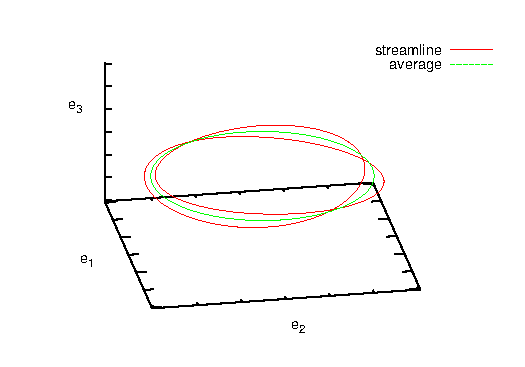
\includegraphics{trefoil_knot.pdf}
%  \caption{
%    A possible streamline (red) with its averaged rotation in green.
%    The streamline was chosen to be a trefoil knot. The reasons for the non-trivial topology are discussed in the text.
%    }
%    \label{fig:particle}
% \end{figure}

%\subsection{Interactions between spinless charges}\label{sec:spinless}
%When an acoustic charge has no spin (or the spin is ignored)
%the equations of motion can be derived from the manifestly gauge invariant energy momentum tensor in  equation \eqnref{TAEM}.
%By taking the  divergence and picking out the spatial terms,
%the force $\vf$ is found to be \cite{Doran2003}
%\begin{align}
%  \vf = - \lr{\rho_q\vE + \vJ \times \vB}.
%\end{align}
%If it is assumed that an acoustic charge $q$ is carried by an `acoustic particle' (a vortex tube without swirl, for instance)
%moving at speed $\vu$, then
%$\vf = - q\lr{\vE + \vu \times \vB}$, which is the Lorentz force law.
%We argue, therefore, that turbulent sources of sound interact according to the Lorentz-force law when measured acoustically.

%Whether this result could be used to model bubble-bubble interactions remains an open question.
%% The force law takes the form
%% \eqal{
%% \dot  u  = - \frac{q}{m_0} F \cdot u
%% }{LorentzGA}
%% when expressed with geometric algebra, where the dot denotes differentiation 
%% with respect to proper time and $m_0$ is the {\em rest mass} of the vortex source,
%% presumably the mass  displaced by the differing density of the vortex.


%% The divergence of the energy momentum tensor gives the force
%% and the spatial component in the lab frame is
%% \begin{align}
%%   \vf = - \lr{\rho_q\vE + \vJ \times \vB}.
%% \end{align}
%% If it is assumed that an acoustic charge $q$ is carried by a `particle' moving at speed $\vu$, then
%% $\vf = - q\lr{\vE + \vu \times \vB}$, which is the Lorentz force law.
%% Turbulent sources of sound, therefore, interact according to the Lorentz-force law when measured acoustically.

%%\subsection{Particles with Spin}


\subsection{Other similar studies}

%The  similarities between acoustics and electromagnetism have long been recognised.
By using a relativistic version of Lighthill's formulation of aeroacoustics it is demonstrated 
that there exists a cosmetic similarity between sound as measured acoustically and electromagnetism. 
We found the acoustic analogue to the electric field is the Lamb vector (proportional to the Coriolis acceleration),
and that the acoustic analogue to the magnetic field is the vorticity.
%The spacetime vorticity tensor takes the role of the field tensor.
An analogy in this form has been presented before by both Marmanis\cite{Marmanis2000} and Sridhar\cite{Marmanis2000,Sridhar1998}.
However, both these attempts were constructed from Galilean fluid mechanics and so the analogy was only partial.
A more complete  analogy, using a relativistic incompressible fluid, was first published by Garrido\cite{Garrido1982} long before the studies of Marmanis and Sridhar.  
Unfortunately, this article was missed by the wider community, 
and has only come to the attention of the author since completing this thesis.
%Nonetheless, the importance of the analogy to ultrasound physics is new.
%To the author's knowledge, the derivation in this report is the first time that the analogy has been  completed.
%The key step, missing in the attempts of Marmanis and Sridhar, 
%is to note that acoustics must be formulated in terms of a Lorentz invariant fluid where
%{\em the speed of sound equals the speed of light}.
%It is only when this step is made that the complete analogy exists for incompressible fluids.
%The motivation for this step is obvious only when it is appreciated that the speed of sound
%may take the role of the speed of light in a relativistic theory.


While the results presented in this chapter make no relation to the speed of light, 
it is worth noting that the formulation carries over unaltered when the speed of sound equals the speed of light.
Relativistic fluids where the sound speed equals the speed of light have been studied many times before
as theoretical curiosities\cite{Taub1978,Pekeris1976, Pekeris1977}.
For example, Pekeris found that Hick's spherical vortex conserves angular momentum if and only if
the sound speed equals the speed of light\cite{Pekeris1977}.
The importance of such fluids, however, has not to the author's knowledge been recognised.
Such fluids map directly to represent {\em what can be measured} when distances are obtained by echo-location.
%Acoustics as measured with ultrasound is therefore {\em identical} to electromagnetism as measured with light.
% With hindsight this correspondence is not too surprising.
% For both acoustics as measured with ultrasound and electromagnetism as measured with light 
% attempt to measure the properties of their propagating signal.
% Both, therefore, 
% represent a similarly limited view of the world,
% the limitations manifesting themselves in the linearity of the equations.

An alternative  analogy between acoustics and special relativity is found in the `acoustic analogue gravity' literature (see Barcel{\'o}, Liberati and Visser\cite{Barcelo2005} for a review).
An {\em acoustic} metric is constructed that describes sound carried in bulk flow.
While the description of space and time in this formulation is Euclidean, the acoustic metric turns out to be pseudo-Euclidean,
and therefore obeys the Lorentz transformation.
This results because  sound carried away by a supersonic flow will never reach us
and so the speed of sound is a limiting velocity in transformations.
The analogue gravity literature then goes on to study the gravitational implications of the acoustic metric.
The acoustic metric, albeit Lorentzian, is not the same as Minkowski's metric used here, 
but is a function of the bulk flow.
Analogue gravity does not consider the measurement process and  operates within a world characterised by two metrics, 
the Lorentz invariant acoustic metric
 and the Galilean invariant spacetime  metric.
The correspondence of analogue gravity with relativity theory is therefore partial.
%The acoustic analogue to special relativity presented here is complete,
%the only difference is that the speed of sound takes the role of the speed of light.


%While the motivations behind the two approaches is similar, in particular the demand that acoustics must be obey a Lorentz invariant metric,
%the approach given here and the approach of analogue gravity are fundamentally different.
%Analogue gravity does not consider the measurement process and so operates within a world characterised by two metrics, 
%the Lorentz invariant acoustic metric (which is a function of the bulk flow)
% and the Galilean invariant spacetime  metric.
%This report argues that only one metric is required;
%the acoustic analogue to special relativity presented here is identical to the original, excepting that is 
%The specPhysics that is measured 
%%Ultrasound measurement demands that the world be described by a Lorentz invariant metric.
%%There is no other way to describe space and time acoustically.
%%In analogue gravity the acoustic metric is Lorentz-invariant, but is not the same as the metric used here.
%%In analogue gravity the metric is a function of the bulk flow,
%%whereas  we argue that this is impossible:
%%the sound speed must be an a priori constant in order to say anything about the world.
%Nevertheless, the success of analogue gravity is very encouraging.
%%Acoustically observed microbubbles could offer an interesting experimental model in this field.




%\section{Discussion}




%\subsection{A problem when modelling with ultrasound}

%\subsection{An alternative view}
%The initial assumption of \secref{}, that the physical description of the medium does not depend on the imaging modality, has been shown to be wrong.
%If we try to derive the quantities of interest, such as the pressure, the temperature, or the density away from the transducer,
%and we use physics derived without ultrasound in mind to do so, 
%then not only do we get the wrong answer, 
%but we get a logical contradiction.

%Getting the wrong answer is not in of itself a problem.  
%If we want to 
%so long as the answer is the derived quantity as mea

%\subsection{Discussion}

%It is at this point that the required constancy of the speed of sound poses some interpretation problems to the acoustic observer,
%for it is well known that the sound speed in a fluid is not in general constant.
%The sound speed is a function of the medium's thermodynamic quantities such as  density, pressure, temperature and entropy,
%and these vary throughout the fluid, not least due to the propagation of the sound wave itself.
%The equations of state that would most naturally be used to characterise a medium often imply a varying sound speed inconsistent with the m%easurement process.
%Conversely, quantities are measurable by ultrasound only if they belong to an equation of state that is consistent with a constant speed of sound.
%The uncomfortable conclusion is that the quantities measured with ultrasound do not in general have the same value as when they are measured with other modalities.
%In ultrasound we speak of the  {\em observable} value rather than the {\em physical} value.

%\section{An illustration}

%%The distinction between the observed and physical value can be illustrated by means of the 
%Let us suppose that we record with ultrasound the compression of a gas with ultrasound - as depicted in \figref{compression}.
%Without using ultrasound, the thermodynamic properties can be measured and are found to fit well the model of an ideal gas.
%That is the pressure, $p$, density, $\rho$ and temperature, $T$, are related by the ideal gas equation
%\eq{
%  p = \rho R T,
%}
%where $R$ is the specific gas constant.

%Changes to the internal energy, $U$, are given by the thermodynamic relation
%\eq{
%  dU =  - pd\rho^{-1} = p \rho^{-2} d\rho = c_v dT
%}
%Using the equation of state we have
%\begin{align}
% p \rho^{-2} d\rho = (c_v/R) (\rho^{-1}dp - p \rho^{-2} d\rho)
%\end{align}
%and so 
%\begin{align}
%c^2 = \gamma p/ \rho = \gamma RT
%\end{align}
%where 
%\begin{align}
%\gamma = (R + c_v)/c_v = c_p/c_v
%\end{align}


%If the chamber is adiabatically compressed, then the gas inside is at a higher pressure and temperature.




%Equations of state that are confirmed by other experimental techniques do not correctly predict the outcomes of ultrasound experiments
%due to ultrasound's incorrect reliance on a constant sound speed.


%It is at this point that the required constancy of the speed of sound poses some interpretation problems to the acoustic observer.




%for it is well known that the sound speed in a fluid is not in general constant.
%The sound speed is a function of the medium's thermodynamic quantities such as  density, pressure, temperature and entropy,
%and these vary throughout the fluid, not least due to the propagation of the sound wave itself.
%Equations of state that are confirmed by other experimental techniques do not correctly predict the outcomes of ultrasound experiments
%due to ultrasound's incorrect reliance on a constant sound speed.





%This is a difficult square to circle.

%One option would be to use ultrasound for the spatio-temporal location of entities, and then ascribe the real, independently measured physical properties and physical laws to those entities.



%One option would be to use ultrasound for the spatio-temporal location of entities, and then ascribe the real, independently measured physical properties and physical laws to those entities.
%An example would be modelling an acoustic medium as an ideal gas; the locations of echos described by \eqnref{radar} and the thermodynamic properties of the medium described by the ideal gas law.
%While this approach seems reasonable it suffers from a lack of internal consistency. 
%An ideal gas heats when compressed, and this alters the speed of sound.  
%Such physics is unmeasurable with ultrasound, even if the underlying model is correct.
%On the one hand the measurement processes assumes that the sound speed is fixed, 
%while on the other the properties of the medium imply that is not.  
%The measurements made with ultrasound will not agree with the predictions of a physically correct model due to ultrasound's reliance on assuming a constant sound speed.


%Put another way, 
%such an approach implies that ultrasound measurement alone cannot measure the properties ascribed in the model.  

%An alternative is to focus on modelling what is measurable - thereby insisting on the internal consistency of the physics.
%Since ultrasound requires that the speed of sound be constant as part of its measurement process, 
%the approach insists that the  model of the medium be consistent with this requirement.
%The equations of state are therefore determined by what can be measured acoustically, 
%rather than driven by what has been shown to be successful in other domains of physics.

%Both approaches are difficult to accept, 
%because in both we have to accept a distinction between 
%Such an approach refute 
%We show in \secref{nonlinear} that this implies that we model fluids with an the adiabatic index of unity.



%Consider for example the acoustic measurement of a compression of the gas in \figref{compression}.
%When the valve compresses the gas the  ideal gas is compressed, it heats up and this increases the speed of sound. 
%However, this change in sound speed is not reflected in the measurement process, and so the physical theory predicted 
%The acoustic measurement processes continues with the original sound speed and so the measured compression is incorrect.  
%The time it takes for a compression phase of the sound wave to return differs from that of the rarefaction.  


%The difficulty with this is that 

% to try to ensure that the underlying thermodynamic properties of the medium are
%If these thermodynamic properties are assumed to take their real, independently measured values then the implied local speed of sound will in general be different than the sound speed assumed in ultrasound.  
%Accordingly, the location where these perturbations are calculated - from their real values - differs from the location that is measured in ultrasound.  
%One would then have to maintain a mapping between what is measured acoustically, with a detailed knowledge of the medium so the real thermodynamic properties can be maintained correct.
%If such a detailed knowledge of the measured medium exists, then the need for acoustic measurement at all is deminished.




%The measured locations of these perturbations will then differ from where the fluctuation actually occured.  In short, we have a contradiction - we ascribe a   valuesare measured independently from the acoustic properties of the medium, 
%then these properties will imply 

%\section{Electro analogy}
%The condition that the sound speed takes the role  of the speed of light
%is enforced by simply equating these two speeds.
%This further requires that the energy density of the fluid, as measured acoustically, be a function of the pressure only (barotropic),
%for the sound speed cannot be set equal to the speed of light otherwise\cite{Taub1978}.

%The complete analogy between an incompressible relativistic fluid and electromagnetism was first published in French by Garrido\cite{Garrido1982} in 1982.
%The results were unknown to the author of this thesis, who derived the results of the following section independently.



%%% Local Variables: 
%%% mode: latex
%%% TeX-master: "../../tshorrock_thesis"
%%% End: 

% LocalWords:  extremum Crocco's
